\documentclass[aspectratio=169,10pt]{beamer}

\usetheme{Madrid}
\usecolortheme{whale}
\useinnertheme{circles}
\setbeamertemplate{navigation symbols}{}
\setbeamertemplate{footline}[frame number]

\usepackage{amsmath,amssymb}
\usepackage{bm}
\usepackage{array}

% ---- notation macros ----
% species-space arrays: upright sans-serif bold
\newcommand{\sa}[1]{\bm{\mathsf{#1}}}
% Cartesian vectors/tensors: bold italic
\newcommand{\ca}[1]{\bm{#1}}
\newcommand{\kB}{k_{\mathrm B}}
\newcommand{\dpa}{\ensuremath{\mathrm{dpa}}}

\setbeamerfont{block title}{size=\small}
\setbeamercolor{block title}{bg=structure!20,fg=black}

\title[SRCD Model in MoDELib2]{The Spatially Resolved Cluster Dynamics (SRCD) Model}
\author[Ghoniem]{N.\ Ghoniem, G.\ Po, M. Marron \& R. Escobar}
\institute[MMS]{Multiscale Materials Solutions --- Deliverable D1/M1}
\date{\today}

\begin{document}

{\setbeamertemplate{footline}{}
\begin{frame}
  \titlepage
  \vspace{-1.2em}
  \footnotesize 
\end{frame}
}

% ---------------- Frame: overview ----------------
\begin{frame}{The SRCD model at a glance}
MoDELib2 represents defect clusters as \textbf{continuum fields}. The model is
\emph{reduced}: it resolves only a few cluster classes explicitly.
\vfill
\begin{columns}[T]
\begin{column}{0.48\textwidth}
\begin{block}{Mobile clusters (\S2.1)}
\small
\begin{itemize}
  \item Small clusters $v,\,i,\,2i,\,3i$
  \item \textbf{Fixed} defect content per cluster
  \item Concentration field $\sa{c}_M$ solved
  \item Governed by a reaction--diffusion \textbf{PDE}
\end{itemize}
\end{block}
\end{column}
\begin{column}{0.48\textwidth}
\begin{block}{Immobile clusters (\S2.2)}
\small
\begin{itemize}
  \item Large clusters $\to$ dislocation \textbf{loops}
  \item Tracked by \textbf{density} $\sa{n}_I$ and \textbf{content} $\sa{c}_I$ only
  \item Size distribution \emph{not} resolved
  \item Governed by coupled \textbf{ODEs}
\end{itemize}
\end{block}
\end{column}
\end{columns}
\vfill
\footnotesize
Interstitial clusters larger than $m_{\max}$ and vacancy clusters larger than
$m_{\min}$ are treated as immobile loops. The mobile and immobile fields exchange
defects with exact mass conservation.
\end{frame}

% ---------------- Frame: notation ----------------
\begin{frame}{Notation: two kinds of non-scalar quantities}
\small
Quantities carry information in \emph{two different spaces}, distinguished by typeface:
\vfill
\begin{center}
\renewcommand{\arraystretch}{1.35}
\begin{tabular}{@{}p{0.30\textwidth} p{0.32\textwidth} p{0.30\textwidth}@{}}
\hline
 & \textbf{Species space} & \textbf{Cartesian space}\\
 & (indexed by $v,i,2i,3i$ or loop family) & (ordinary 3D vectors/tensors)\\
\hline
Typeface & upright sans-serif bold & bold italic\\
Vectors (lowercase) & $\sa{c}_M,\ \sa{J},\ \sa{S}_{vL}$ & $\ca{J}_x,\ \ca{\nabla},\ \ca{\sigma}$\\
Matrices (uppercase) & $\sa{D},\ \sa{E},\ \sa{R}_2$ & $\ca{D}_x$ (diffusion tensor)\\
\hline
\end{tabular}
\end{center}
\vfill
Entries of the species-space flux $\sa{J}$ are \emph{themselves} Cartesian vectors
$\ca{J}_x$, and the divergence $\ca{\nabla}\!\cdot$ acts on each entry:
\[
\sa{J}=\big[\,\ca{J}_v,\ \ca{J}_i,\ \ca{J}_{2i},\ \ca{J}_{3i}\,\big]^{\mathsf T},
\qquad
\ca{J}_x=-\ca{D}_x\,\ca{\nabla} c_x .
\]
\end{frame}

% ---------------- Frame: mobile definitions ----------------
\begin{frame}{Mobile species: definitions}
\small
Mobile clusters are set by \texttt{mobileSpeciesVector}. Example \texttt{Zr\_CD4.txt}:
\[
\texttt{mobileSpeciesVector} = -1\ \ 1\ \ 2\ \ 3
\ \Rightarrow\ \{v,\ i,\ 2i,\ 3i\}.
\]
Collected into the \emph{signed}-size array $\sa{m}_M$ with polarity $p_k$:
\[
\sa{m}_M=[-1,+1,+2,+3]^{\mathsf T},\quad
\sa{p}_M=[-1,+1,+1,+1]^{\mathsf T},\quad
p_k=\frac{m_k}{|m_k|}\in\{+1,-1\}.
\]
\begin{itemize}
  \item $p_k=+1$: interstitial character; \ $p_k=-1$: vacancy character; \ $|m_k|$ = number of point defects.
  \item Boolean selectors: \ $\sa{M}_i=\tfrac12(1+\sa{p}_M)$, \quad $\sa{M}_v=\tfrac12(1-\sa{p}_M)$.
  \item Mobile concentration field (per-atom, fractional): \ $\sa{c}_M=[c_v,c_i,c_{2i},c_{3i}]^{\mathsf T}$.
\end{itemize}
\vfill
\centering
\footnotesize Point-defect fluxes feeding the loop coupling:\quad
$\phi_v=\omega_v c_v$, \qquad $\phi_i=\omega_i\,(c_i+2c_{2i}+3c_{3i})$.
\end{frame}

% ---------------- Frame: master PDE ----------------
\begin{frame}{Mobile master equation (steady-state reaction--diffusion PDE)}
\begin{block}{}
\[
\boxed{\;
0=-\,\ca{\nabla}\!\cdot\sa{J}
\;+\;\sa{P}_M
\;+\;\tfrac12\big(\sa{I}\otimes\sa{c}_M^{\mathsf T}\big)\sa{R}_2\,\sa{c}_M
\;+\;(\sa{E}-\sa{D})\,\sa{c}_M
\;+\;\sa{S}_{vL}
\;}\tag{1}
\]
\end{block}
\small
\begin{tabular}{@{}ll@{}}
$-\ca{\nabla}\!\cdot\sa{J}$ & diffusive transport of the four mobile species\\[2pt]
$\sa{P}_M=G\varepsilon\,\sa{f}$ & cascade production ($G$ = \dpa\ rate, $\varepsilon$ survival, $\sa{f}$ partition) \hfill (4)\\[2pt]
$\tfrac12(\sa{I}\otimes\sa{c}_M^{\mathsf T})\sa{R}_2\sa{c}_M$ & second-order reactions (clustering of two mobile species); $x$-entry $=\tfrac12\sa{c}_M^{\mathsf T}\sa{R}_2^{x}\sa{c}_M$\\[2pt]
$\sa{E}\,\sa{c}_M$ & thermal dissociation (emission) of mobile clusters \hfill (9)\\[2pt]
$-\sa{D}\,\sa{c}_M$ & annihilation at immobile sinks (network + loops) \hfill (11)\\[2pt]
$\sa{S}_{vL}$ & vacancies returned from dissolving/emitting vacancy loops \hfill (58)\\
\end{tabular}
\vfill
\footnotesize $\sa{I}$ is the $4\times4$ identity; $\otimes$ the Kronecker product. Component-wise,
(1) reproduces the 0D \texttt{ZrMicro} rate equations term by term.
\end{frame}

% ---------------- Frame: rate constants ----------------
\begin{frame}{Reaction rates, emission, and mobility}
\small
\textbf{Pairwise reaction rate} between species $m,n$ (built from summed jump frequencies):
\[
\beta_{m,n}=A_{m,n}\,\Omega^{|\mathsf M_m\mathsf M_n|}\,(D_m+D_n)(r_m+r_n)
\;=\;(\omega_m+\omega_n),\tag{6,7}
\]
consistent with the 0D form $R_{a,b}=(\omega_a+\omega_b)C_aC_b$; the $i$--$v$ channel carries the
recombination factor $\beta_r$.
\vfill
\textbf{Thermal emission} (dissociation) rate from detailed balance:
\[
\alpha_{m,n}=\beta_{m,n}\,\exp\!\Big(-\tfrac{E^{b}_{m,n}}{\kB T}\Big),
\qquad E^b_{m,n}=\text{binding energy of the }(m{+}n)\text{ cluster}.\tag{10}
\]
\vfill
\textbf{Jump frequency / diffusivity} and \textbf{capture radius}:
\[
\omega_x=z_c\nu_x\exp\!\Big(\!-\tfrac{E^m_x}{\kB T}\Big),\quad
(\ca{D}_x)_{ij}=(D^0_x)_{ij}\exp\!\Big(\!-\tfrac{E^{xm}_{ij}}{\kB T}\Big),\quad
r_m=\!\begin{cases}\big(\tfrac{3\Omega_0}{4\pi}\big)^{1/3}, & |m_m|=1\\[3pt]\big(\tfrac{|m_m|\Omega_0}{\pi b}\big)^{1/2}, & |m_m|>1.\end{cases}\tag{8}
\]
\end{frame}

% ---------------- Frame: sinks, bias, BCs ----------------
\begin{frame}{Sinks, loop bias, and boundary conditions}
\small
\textbf{Mobile-to-immobile reaction matrix} $=$ network sinks $+$ loop absorption:
\[
\sa{D}=\operatorname{diag}\{\sa{\omega}\odot\sa{C}_s\}+\sa{D}_d\,\sa{K}_L,
\qquad
\sa{K}_L=\operatorname{diag}\{\sa{k}^2\},\quad
k^2_m=\sum_{I_L} k^2_{I_L,m}. \tag{11,12}
\]
Partial loop sink strengths use per-family bias factors $Z^m_{I_L}$, radii $r_{I_L}$, densities $n_{I_L}$
(e.g. $k^2_{a_L,m}=Z^m_{a_L,\mathrm{tot}}\,2\pi r_{a_L}n_{a_L}$). \hfill (13--15)
\vfill
\textbf{Diffusional-anisotropy-difference (DAD) bias} — emerges naturally from the tensorial flux:
\[
Z^{\mathrm{DAD},0}_{a_L,m}=Z^0_m\frac{p_m+(p_m)^{-2}}{2},\quad
Z^{\mathrm{DAD},0}_{c_L,m}=Z^0_m\,p_m,\quad
p_m=\big(D^c_m/D^a_m\big)^{1/6}.\tag{16}
\]
\vfill
\textbf{Boundary condition} (Dirichlet perfect sink; Robin generalization in the report):
\[
\sa{c}_M(\ca{x})=\sa{c}_{\mathrm{bnd,eq}}(\ca{x}),\qquad
c^k_{\mathrm{bnd,eq}}=c^k_0\exp\!\Big(\!-\tfrac{m_k t_n\Omega}{\kB T}\Big),\quad
c^k_0=|m_k|\exp\!\Big(\!-\tfrac{E^f_k+m_k q\,\Omega^r_k}{\kB T}\Big).\tag{20--22}
\]
\end{frame}

% ---------------- Frame: immobile definitions ----------------
\begin{frame}{Immobile loops: families, fields, and geometry}
\small
Four loop families (one vacancy $\langle c\rangle$ loop, three prismatic $\langle a\rangle$ interstitial loops):
\[
\mathsf L=\{vL,\ ia_1,\ ia_2,\ ia_3\},\qquad
p_{vL}=-1,\ \ p_{ia_1}=p_{ia_2}=p_{ia_3}=+1.\tag{23,24}
\]
Each family carries two per-atom fields — \textbf{density} $\sa{n}_I$ and \textbf{content} $\sa{c}_I$:
\[
\sa{n}_I=[n_{vL},n_{ia_1},n_{ia_2},n_{ia_3}]^{\mathsf T},\quad
\sa{c}_I=[c_{vL},c_{ia_1},c_{ia_2},c_{ia_3}]^{\mathsf T},\quad
\bar m_k=\frac{c_k}{n_k},\quad
r_k=\ell_k\sqrt{\tfrac{c_k}{n_k}}.\tag{25--28}
\]
\vfill
\textbf{Shape transition} — vacancy clusters morph from a compact bi-pyramid to a planar loop via a
sigmoid $S_k(m_k)$:
\[
R_k=\big(1-S_k\big)R^{\mathrm{pyr}}_k+S_k R^{\mathrm{loop}}_k,\qquad
S_k(m_k)=\frac{1}{1+\exp\!\big(-\frac{m_k-m^0_k}{w_k}\big)}.\tag{29,31}
\]
The same $S_k$ interpolates the formation-volume tensor $\Omega_k$ between pyramid and loop limits. \hfill (33,34)
\end{frame}

% ---------------- Frame: density ODE ----------------
\begin{frame}{Loop density evolution}
\begin{block}{}
\[
\frac{d\sa{n}_I}{dt}=\dot{\sa{N}}_{\mathrm{nuc}}-\sa{a}_n-\sa{\Delta}_N .\tag{35}
\]
\end{block}
\small
\textbf{Nucleation} — interstitial loops from clustering $+$ cascade seed; vacancy loops from cascade only:
\[
\dot{\sa{N}}_{\mathrm{nuc}}=\sa{w}(\ca{\sigma})\,\Phi_{\mathrm{clus}}+\sa{G}_L\oslash\sa{n}_{\mathrm{nuc}},
\qquad \Phi_{\mathrm{clus}}=R_{i,3i}+R_{2i,2i}.\tag{37}
\]
Stress-biased orientation weights (small-stress limit of SIPN):
\[
w_{a_k}(\ca{\sigma})=\tfrac13(1+\chi\,\hat\sigma_{kk}),\quad \textstyle\sum_k w_{a_k}=1,\qquad
\chi^k_i=\frac{\exp(\ca{\sigma}:\Omega_k/\kB T)\,I^k_i}{\sum_p \exp(\ca{\sigma}:\Omega_p/\kB T)\,I^p_i}.\tag{38}
\]
\vfill
\textbf{Annealing} (vacancy loops only) and \textbf{coalescence} (like-loop $+$ loop--network channels):
\[
\sa{a}_n=\Big[\tfrac{n_{vL}}{\tau_{vL}},0,0,0\Big]^{\mathsf T},\ \
\tau_{vL}=\tau^0_{vL}e^{E^a_{vL}/\kB T};\qquad
\Delta_N^k=\big(\nu^k_{LL}\phi^k_{LL}+\nu^k_{LN}\phi^k_{LN}\big)n_k.\tag{36,39}
\]
\end{frame}

% ---------------- Frame: content ODE ----------------
\begin{frame}{Loop content evolution and defect conservation}
\begin{block}{}
\[
\frac{d\sa{c}_I}{dt}=\dot{\sa{G}}_c+\sa{P}_G+\sa{s}_{\mathrm{nuc}}-\sa{A}_c-\sa{\Delta}_C .\tag{40}
\]
\end{block}
\small
\textbf{Mass-conserving growth} — each family captures its like defect, recombines with the opposite,
weighted by DAD$+$SIPA capture efficiencies $Z^{k}_m(\ca{\sigma})$:
\[
\dot G^c_{vL}=p_{vL}\pi_{vL}\big(Z^{vL}_v\phi_v-Z^{vL}_i\phi_i\,g(r_{vL})\big),\quad
\dot G^c_{a_kL}=p_{a_kL}\pi_{a_kL}\big(Z^{a_kL}_i\phi_i-Z^{a_kL}_v\phi_v\big).\tag{43--51}
\]
\textbf{Cascade deposition}, \textbf{nucleation seeding}, \textbf{thermal emission} of the mean-size vacancy loop:
\[
\sa{P}_G=G\big(\varepsilon_{ia}\sa{w}(\ca{\sigma})+\varepsilon_{vL}\sa{w}'\big),\quad
N_c=4R_{i,3i}+2R_{2i,2i}+3R_{2i,3i},\quad
\alpha_{v,vL}(\bar m)=\beta_{v,vL}e^{-E^b_{v,vL}(\bar m)/\kB T}.\tag{52,53,56}
\]
\vfill
\begin{block}{Exact conservation}
\footnotesize
Vacancies released by dissolution ($\sa{A}_c$) and emission ($\sa{A}^{\mathrm{emit}}_c$) feed the mobile pool
via $\sa{S}_{vL}$ (Eq.~58), term-by-term identical to the loop debit. Every defect lost to a loop through
$\sa{D}$ is credited exactly once — \textbf{no double counting}.
\end{block}
\end{frame}

% ================= Model Calibration =================
\section{Model Calibration}

\begin{frame}{Calibration: $\langle a\rangle$-loop density vs.\ experiment}
\centering
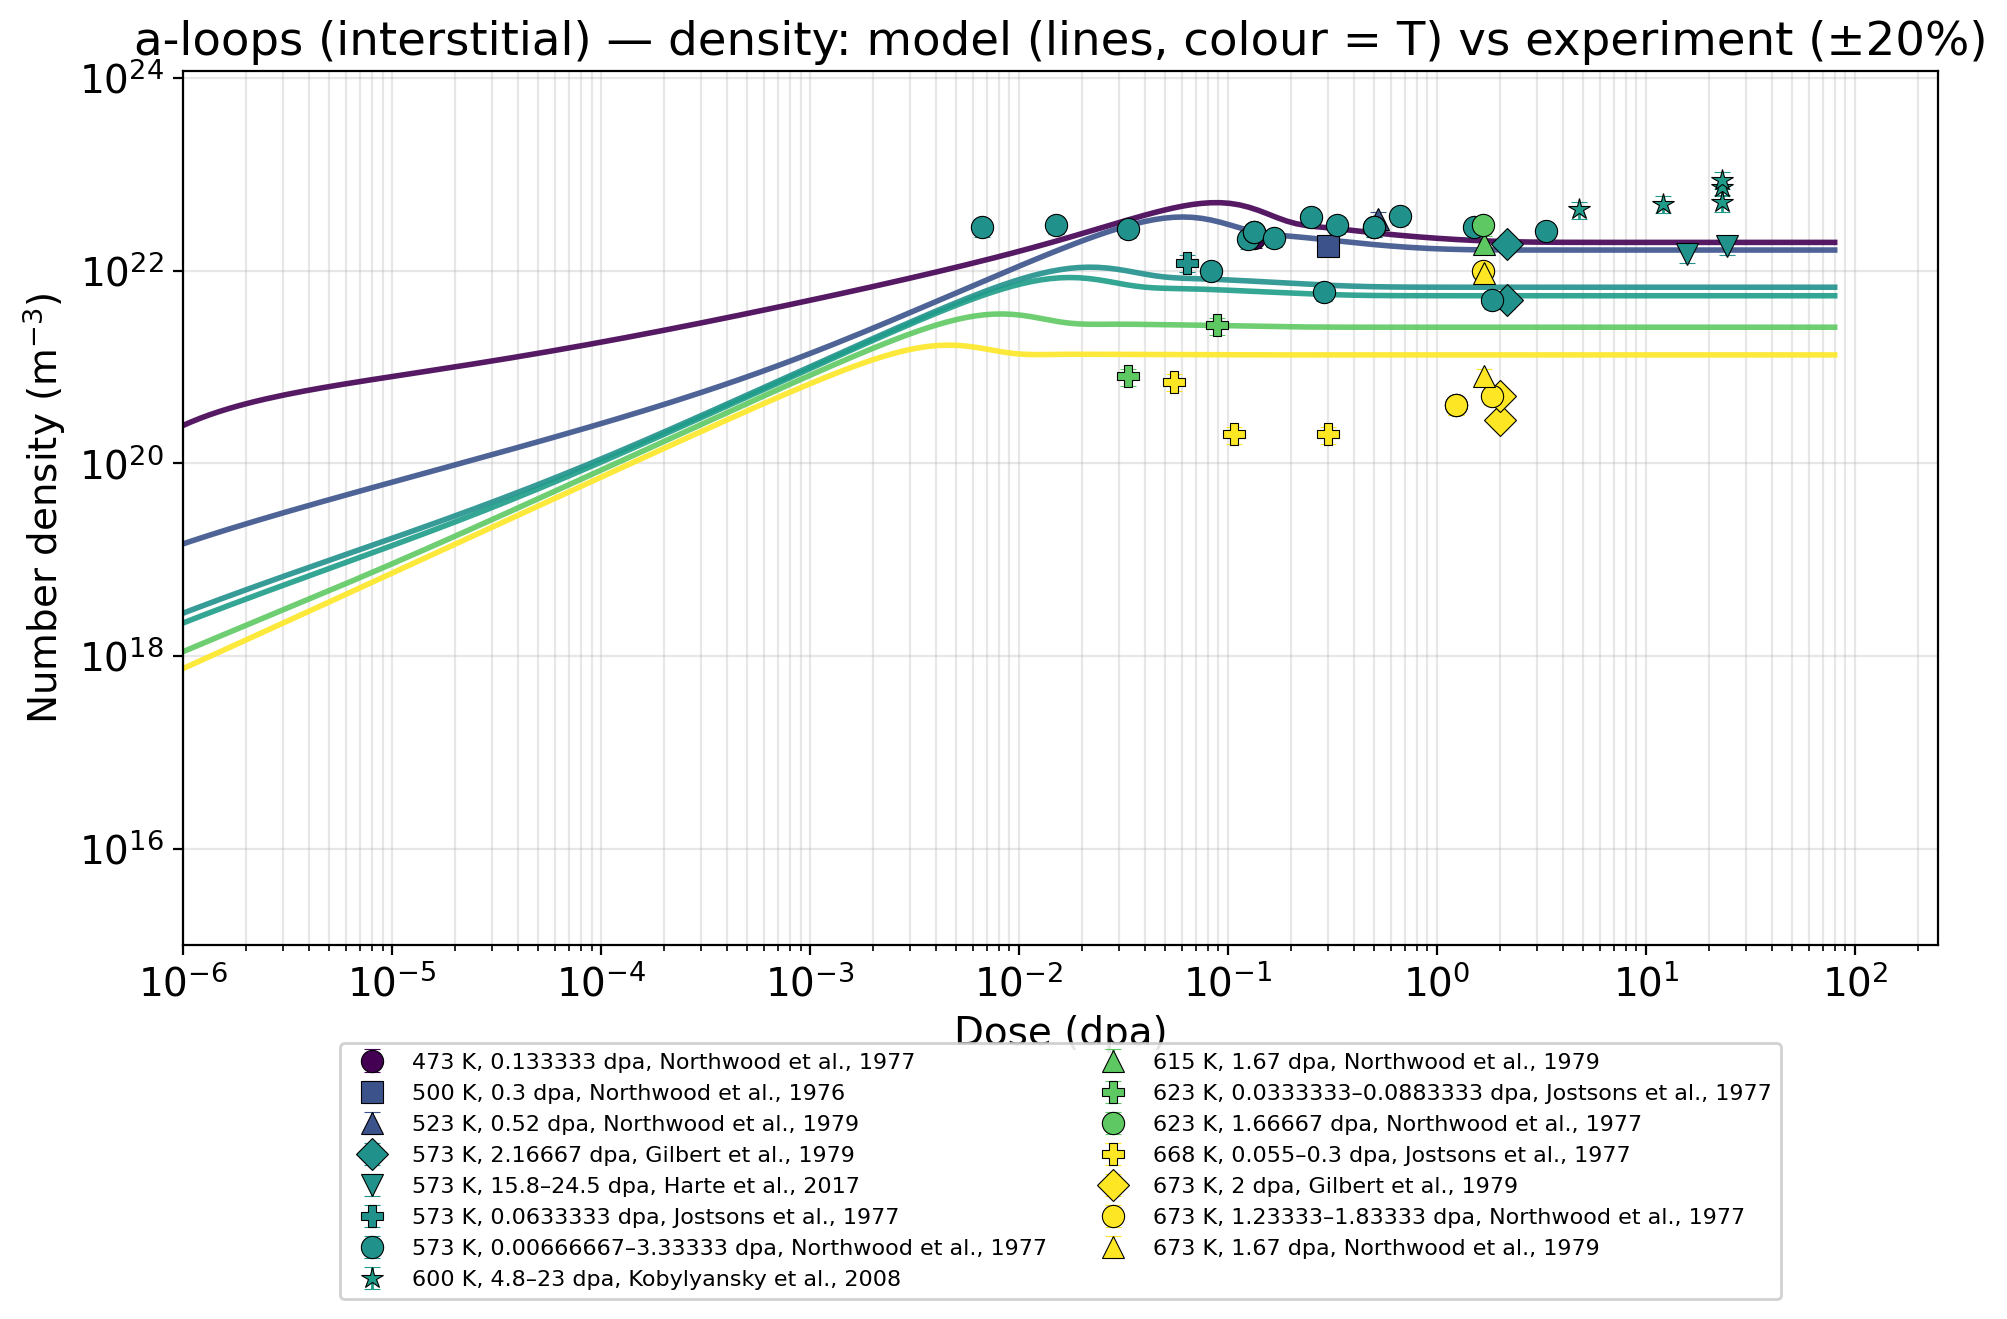
\includegraphics[width=0.85\linewidth,height=0.72\textheight,keepaspectratio]{figures/aloop_density_vs_experiment.png}\\[4pt]
\footnotesize Interstitial $\langle a\rangle$-loop number density vs.\ dose, model against the
experimental database. The prediction saturates near $4\times10^{21}\,\mathrm{m^{-3}}$, at the
lower edge of the measured Zr band ($\sim\!1$--$3\times10^{22}\,\mathrm{m^{-3}}$), consistent
with the conservative coalescence rate.
\end{frame}

\begin{frame}{Calibration: $\langle c\rangle$-loop density vs.\ experiment}
\centering
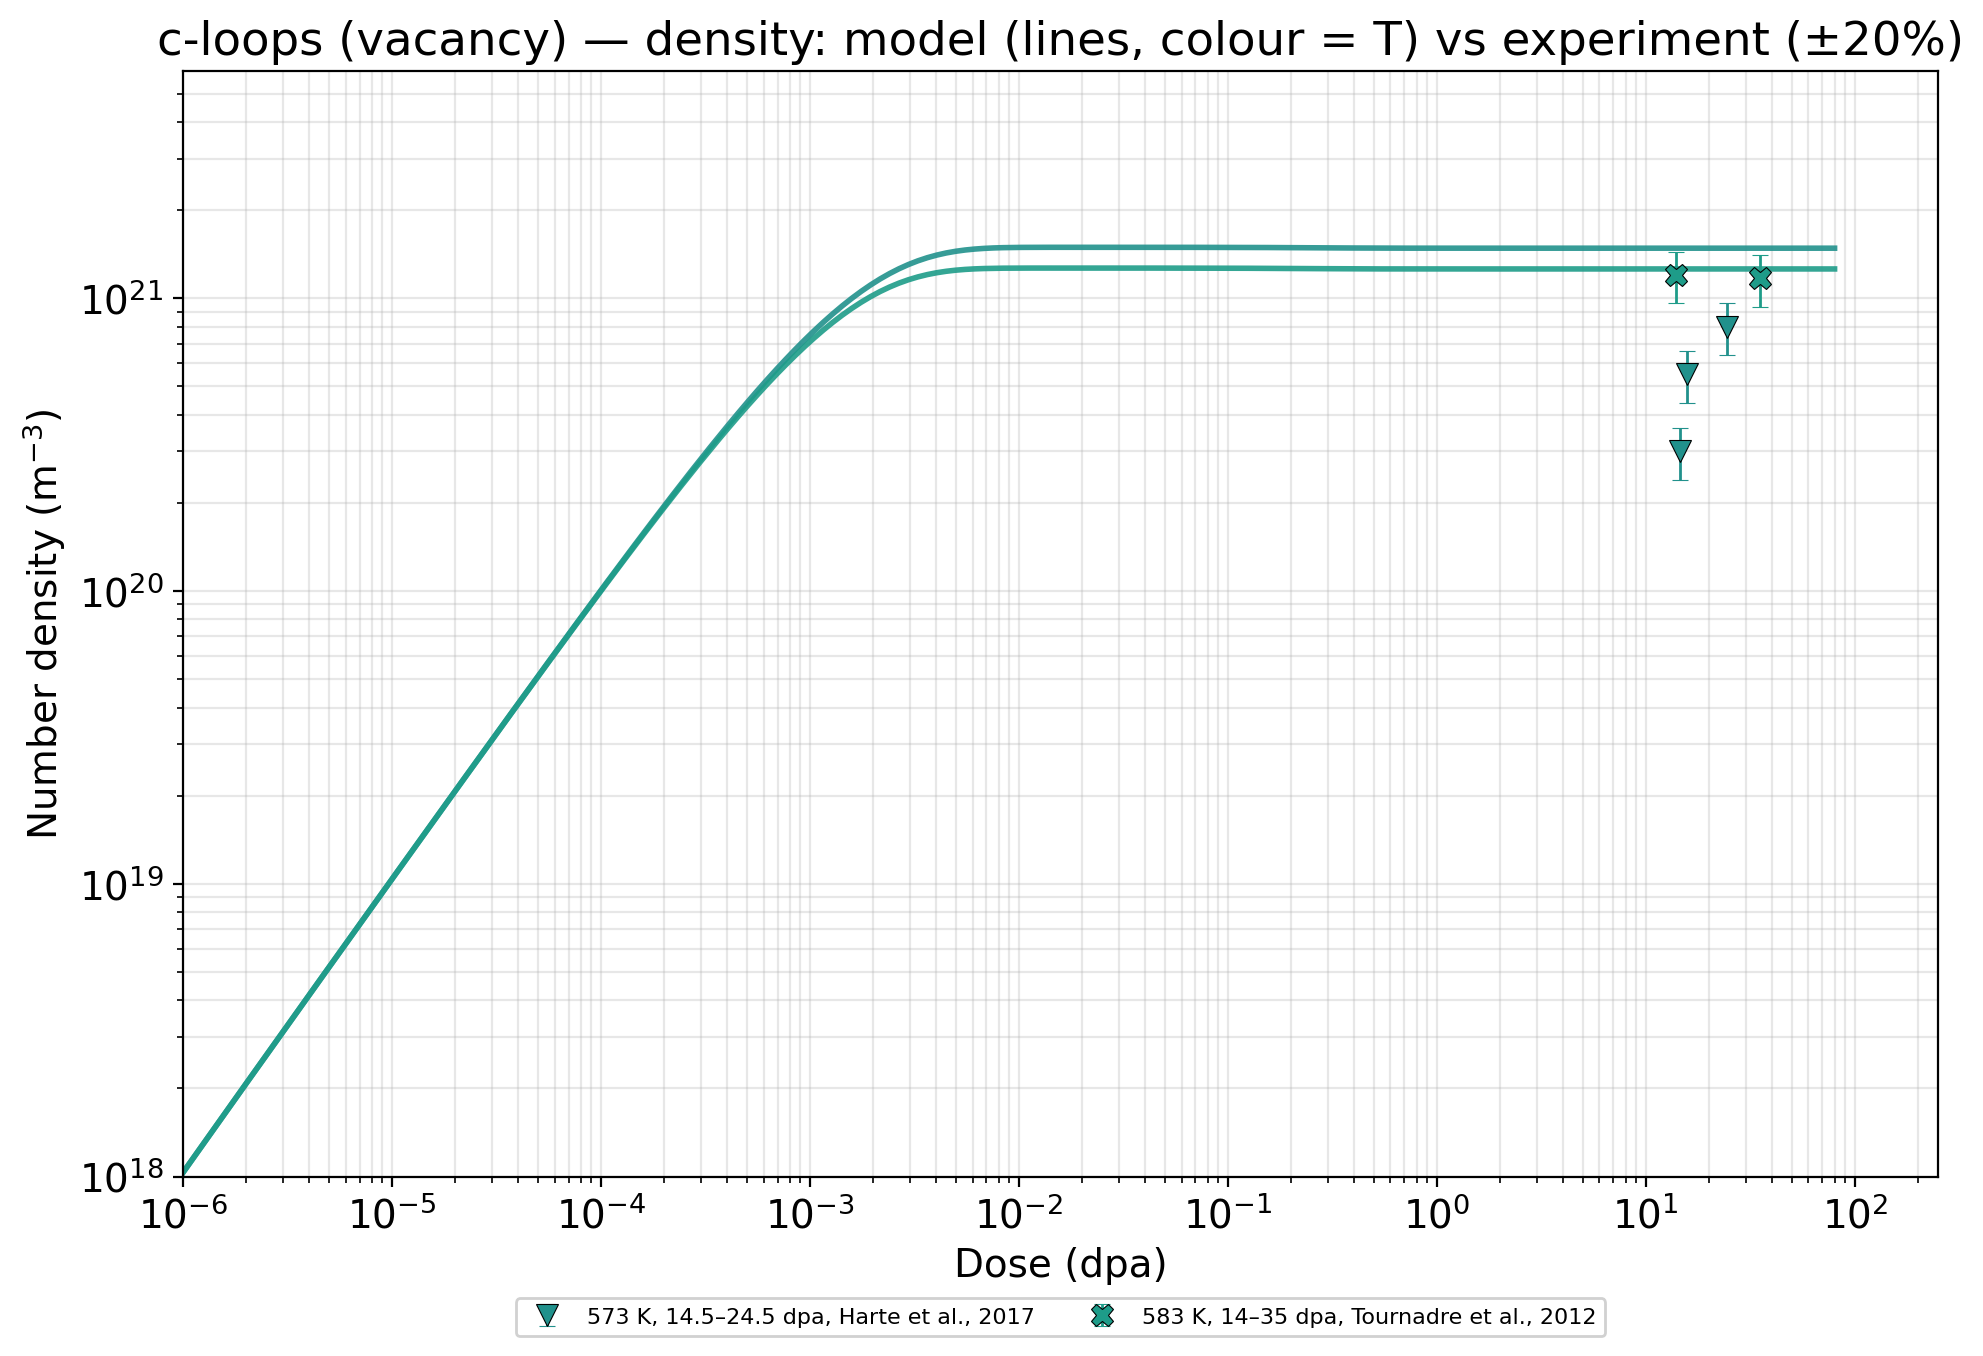
\includegraphics[width=0.85\linewidth,height=0.72\textheight,keepaspectratio]{figures/cloop_density_vs_experiment.png}\\[4pt]
\footnotesize Vacancy $\langle c\rangle$-loop number density vs.\ dose against experiment. The
predicted density saturates near $10^{21}\,\mathrm{m^{-3}}$; consistent with the anisotropic-bias
picture, vacancy loops dominate the stored volume while staying below the interstitial loops in number.
\end{frame}

\begin{frame}{Calibration: $\langle a\rangle$-loop diameter vs.\ experiment}
\centering
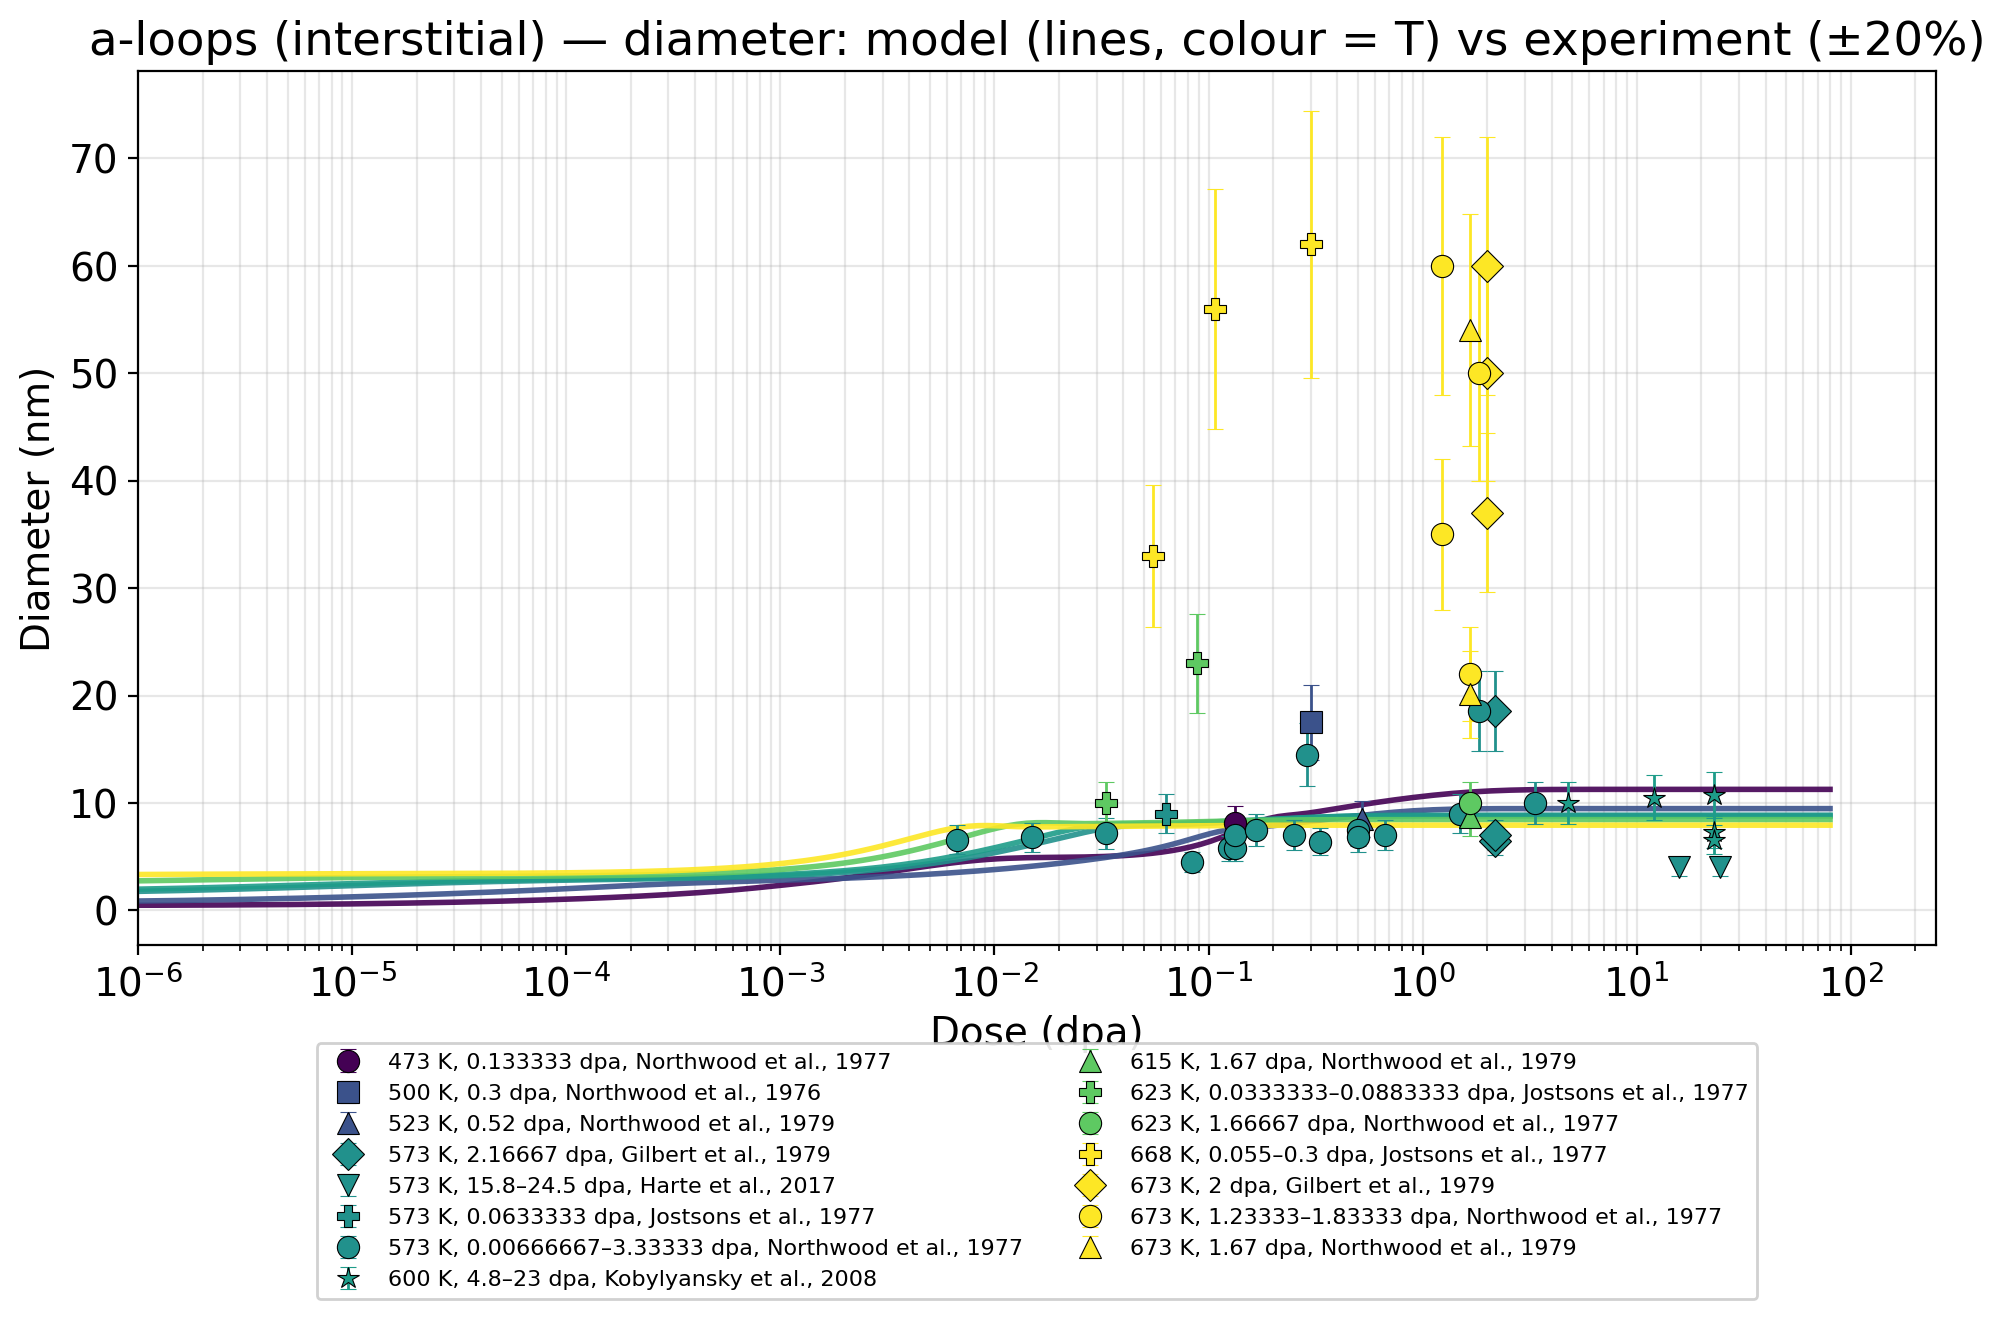
\includegraphics[width=0.85\linewidth,height=0.72\textheight,keepaspectratio]{figures/aloop_diameter_vs_experiment.png}\\[4pt]
\footnotesize Mean $\langle a\rangle$-loop diameter vs.\ dose compared with experiment. The model
saturates near $9$--$10\,$nm, in good agreement with the bulk of the low- and mid-temperature
measurements.
\end{frame}

\begin{frame}{Calibration: $\langle c\rangle$-loop diameter vs.\ experiment}
\centering
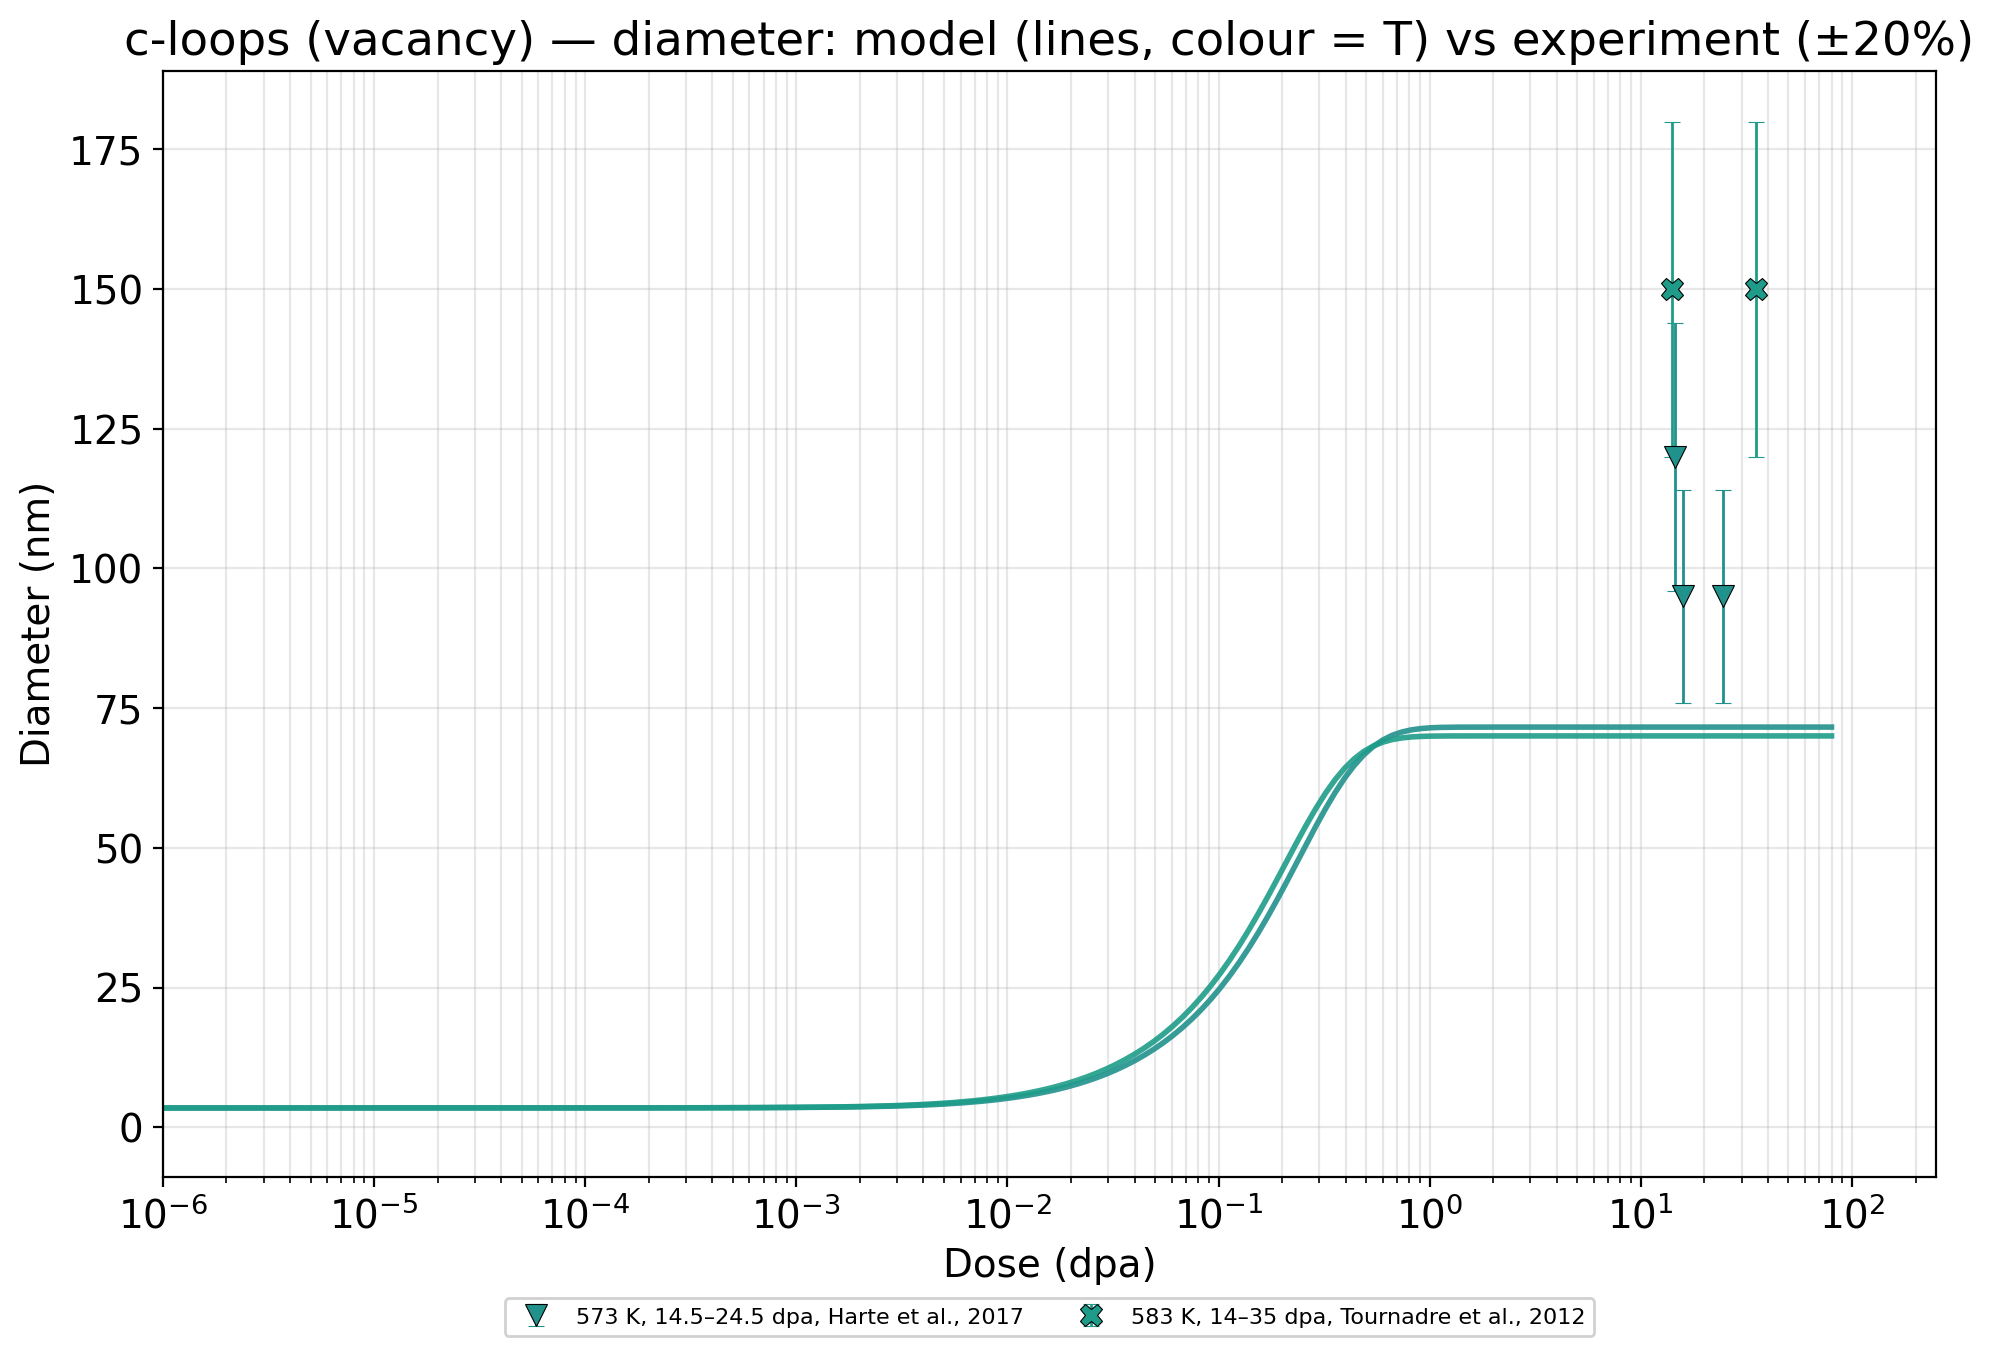
\includegraphics[width=0.85\linewidth,height=0.72\textheight,keepaspectratio]{figures/cloop_diameter_vs_experiment.png}\\[4pt]
\footnotesize Mean $\langle c\rangle$-loop diameter vs.\ dose against experiment. The prediction
rises after $\sim\!10^{-1}\,$dpa toward $\sim\!70\,$nm and under-predicts the measured
$95$--$150\,$nm sizes (Harte, $573\,$K; Tournadre, $583\,$K) by $\sim\!1.5$--$2\times$ --- the
principal discrepancy motivating the targeted $c$-loop refit.
\end{frame}


% ================= Simulation Results =================
\section{Simulation Results}

\begin{frame}{Mobile point-defect fields}
\centering
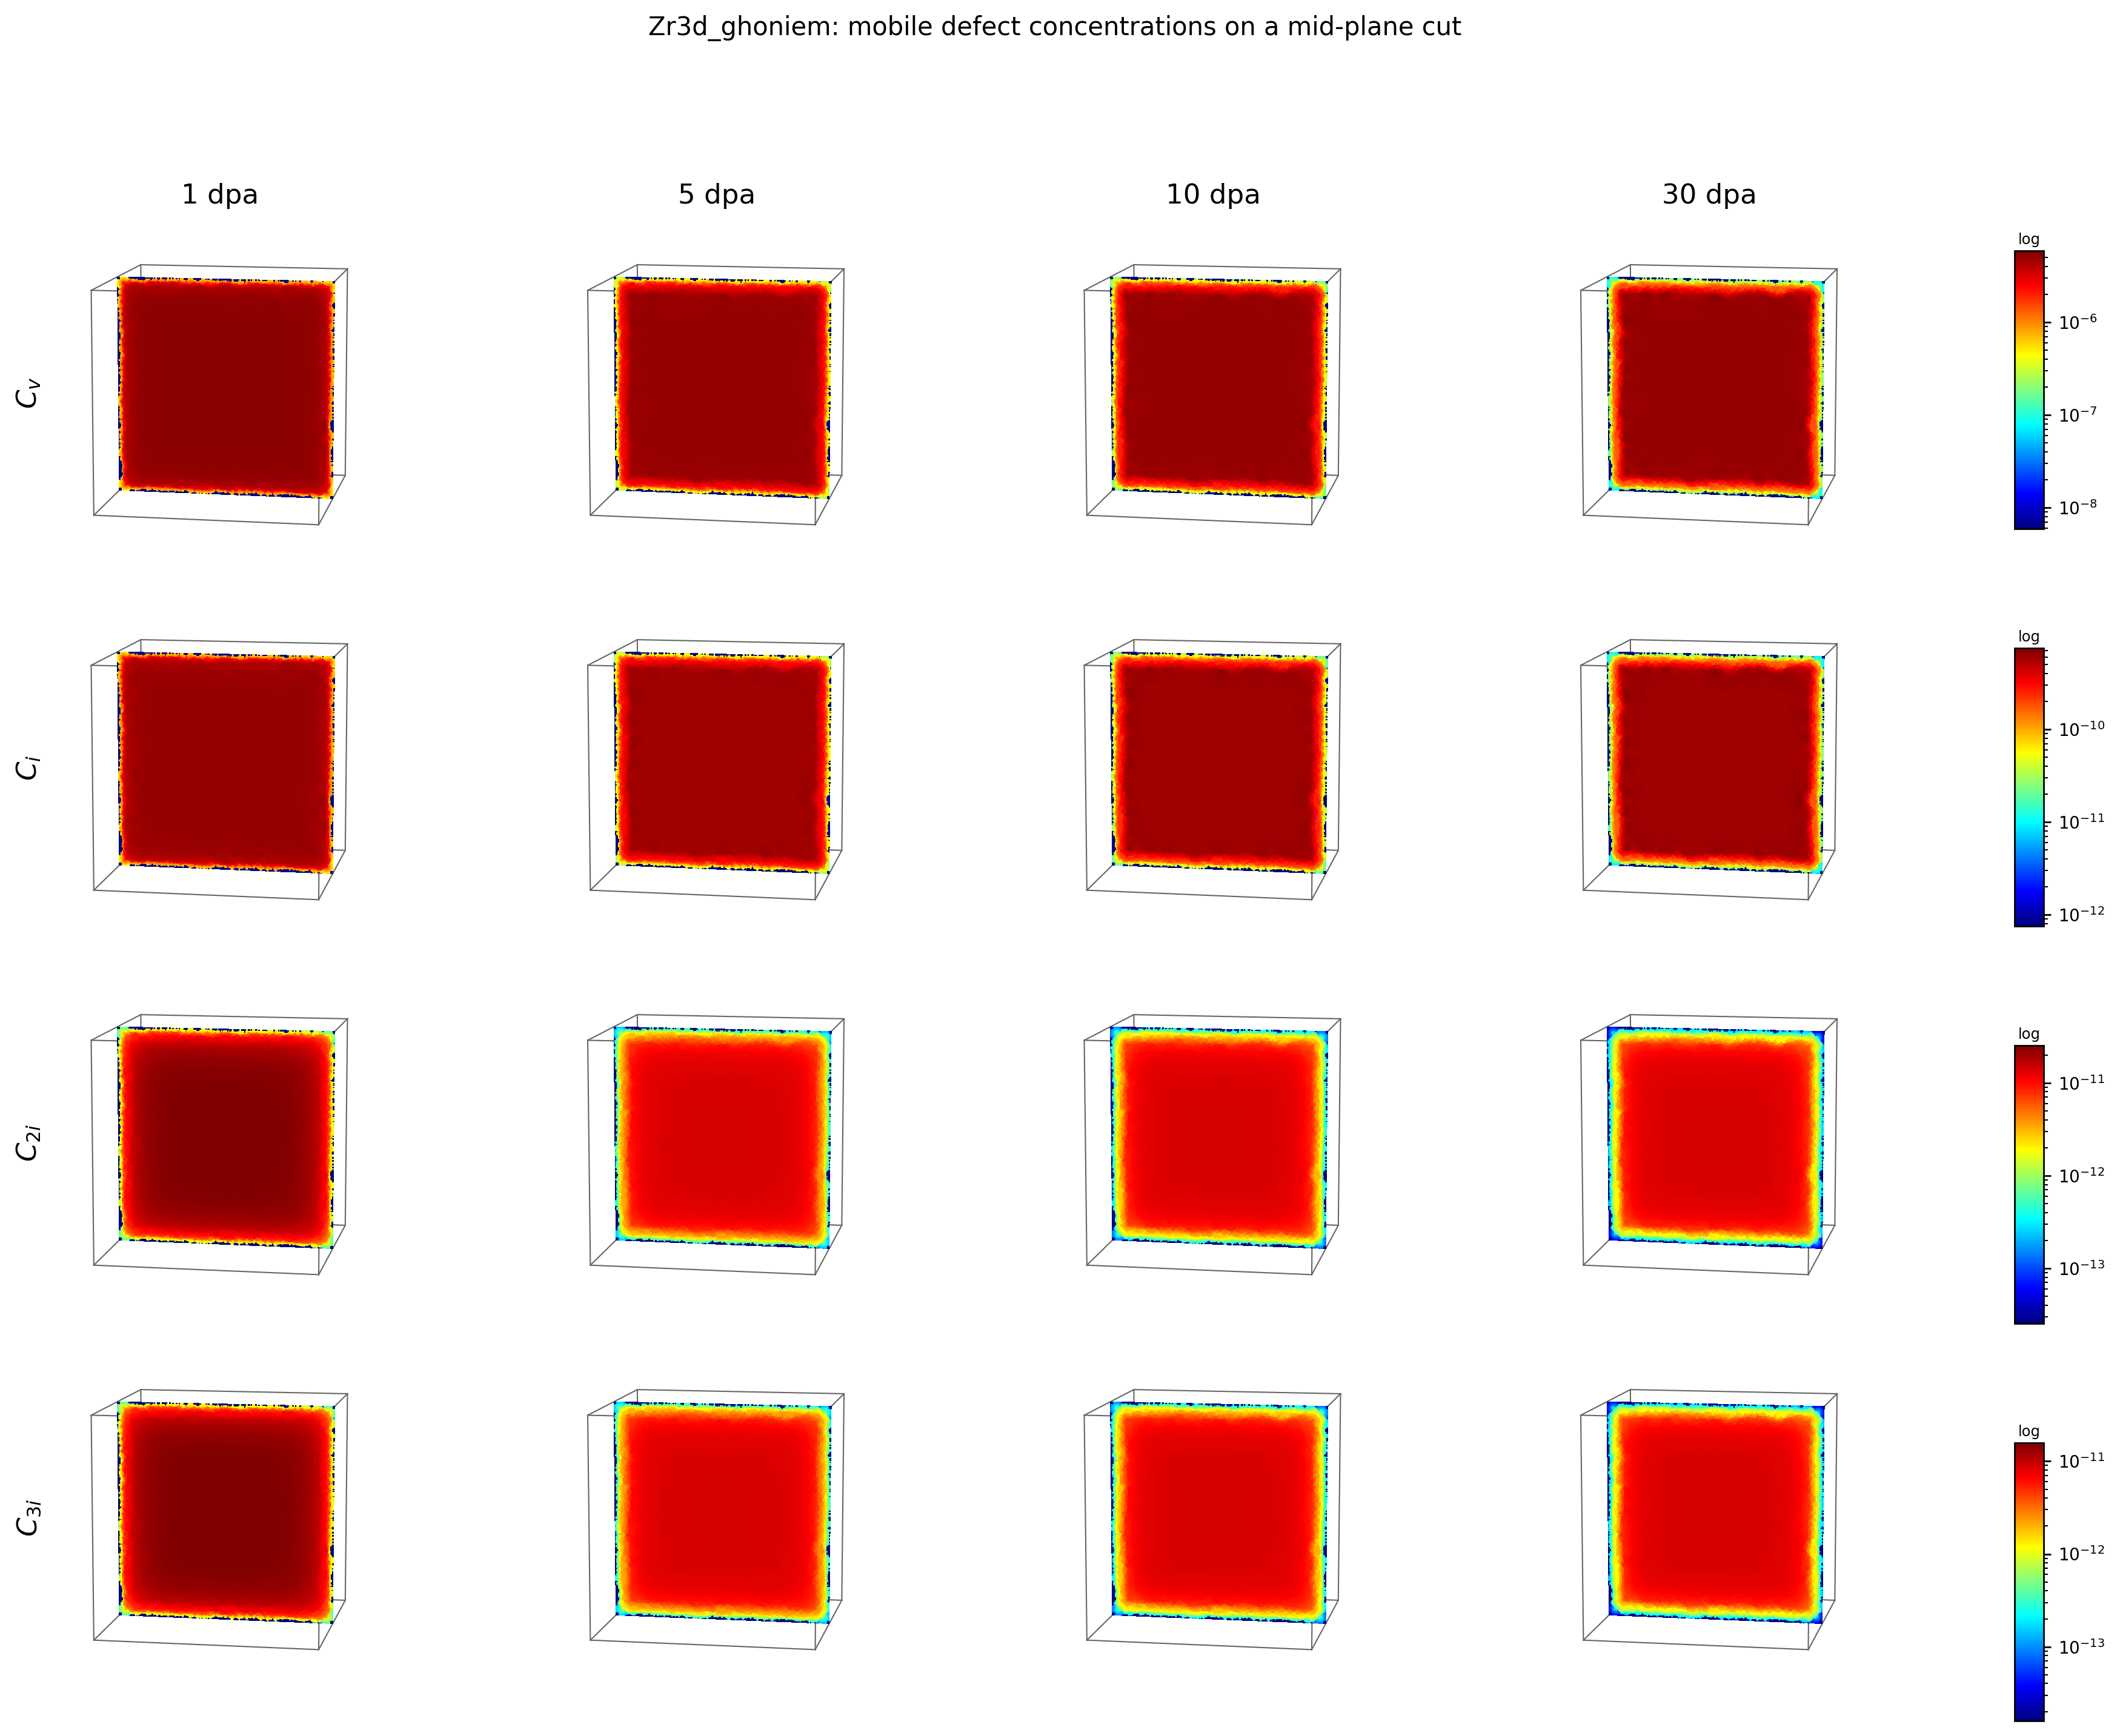
\includegraphics[width=0.85\linewidth,height=0.72\textheight,keepaspectratio]{figures/mobile_fields.png}\\[4pt]
\footnotesize Steady-state concentration fields of the mobile species — vacancies $C_v$, mono-interstitials $C_i$, and small interstitial clusters $C_{2i}$ and $C_{3i}$ — on a mid-plane cut at $1$, $5$, $10$, and $30\,$dpa. All species are nearly uniform in the grain interior and depleted toward the grain boundaries.
\end{frame}

\begin{frame}{$\langle a\rangle$-loop population: family~1}
\centering
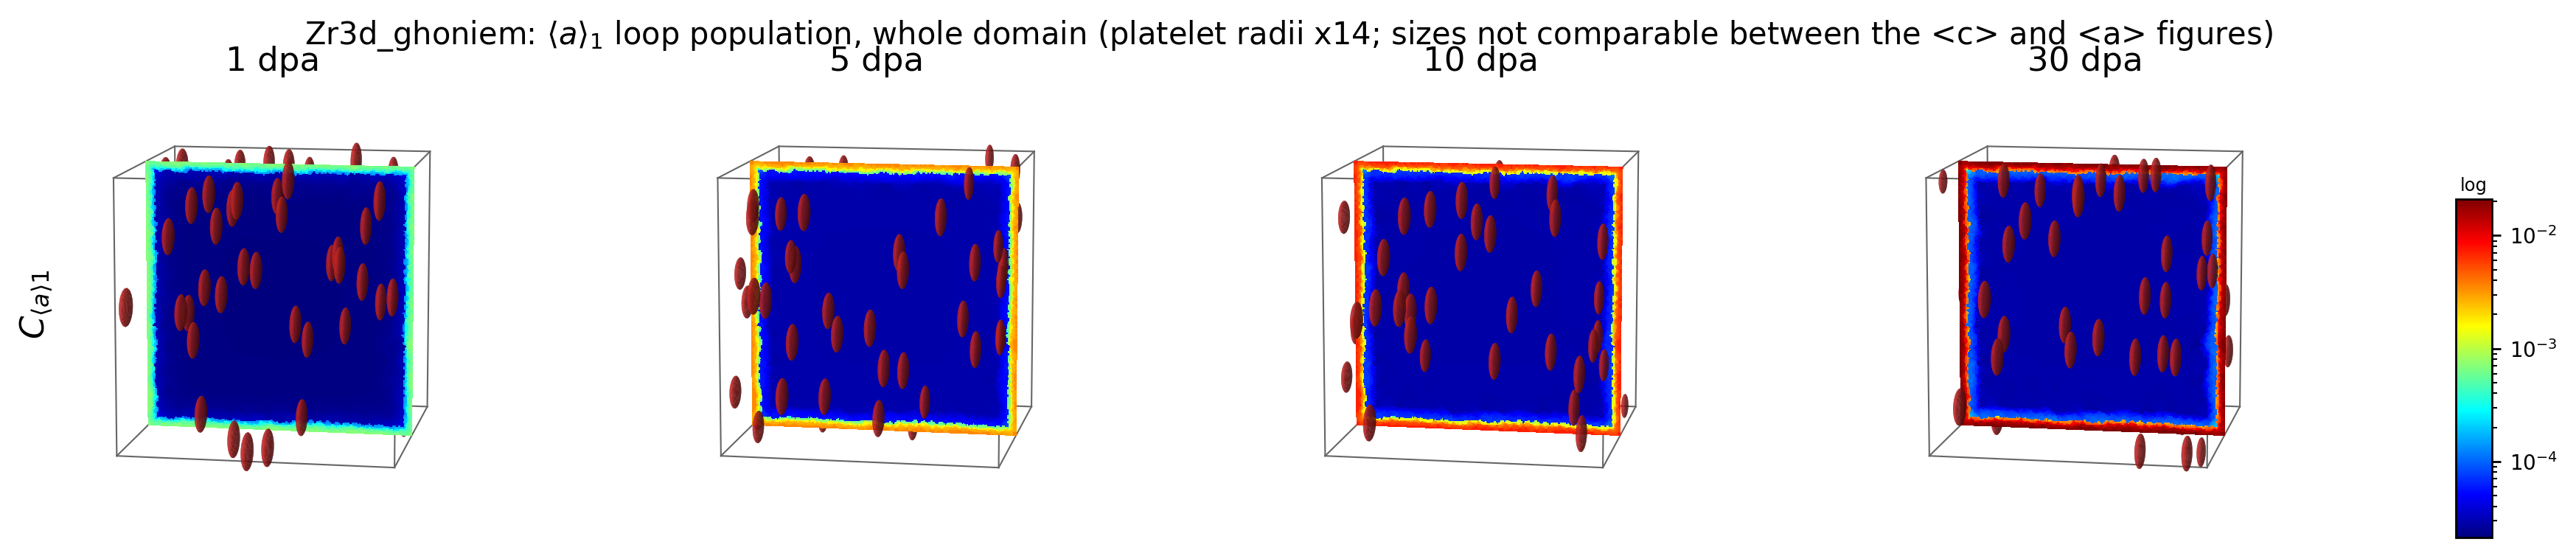
\includegraphics[width=0.85\linewidth,height=0.72\textheight,keepaspectratio]{figures/loops_a1_overlay.png}\\[4pt]
\footnotesize Spatial population of the first $\langle a\rangle$-loop family $C_{(a)1}$ over the whole domain at $1$--$30\,$dpa (platelet markers scaled $\times14$, log colour scale). Loops nucleate throughout the interior and coarsen with dose while the boundary layer stays depleted.
\end{frame}

\begin{frame}{$\langle a\rangle$-loop population: family~2}
\centering
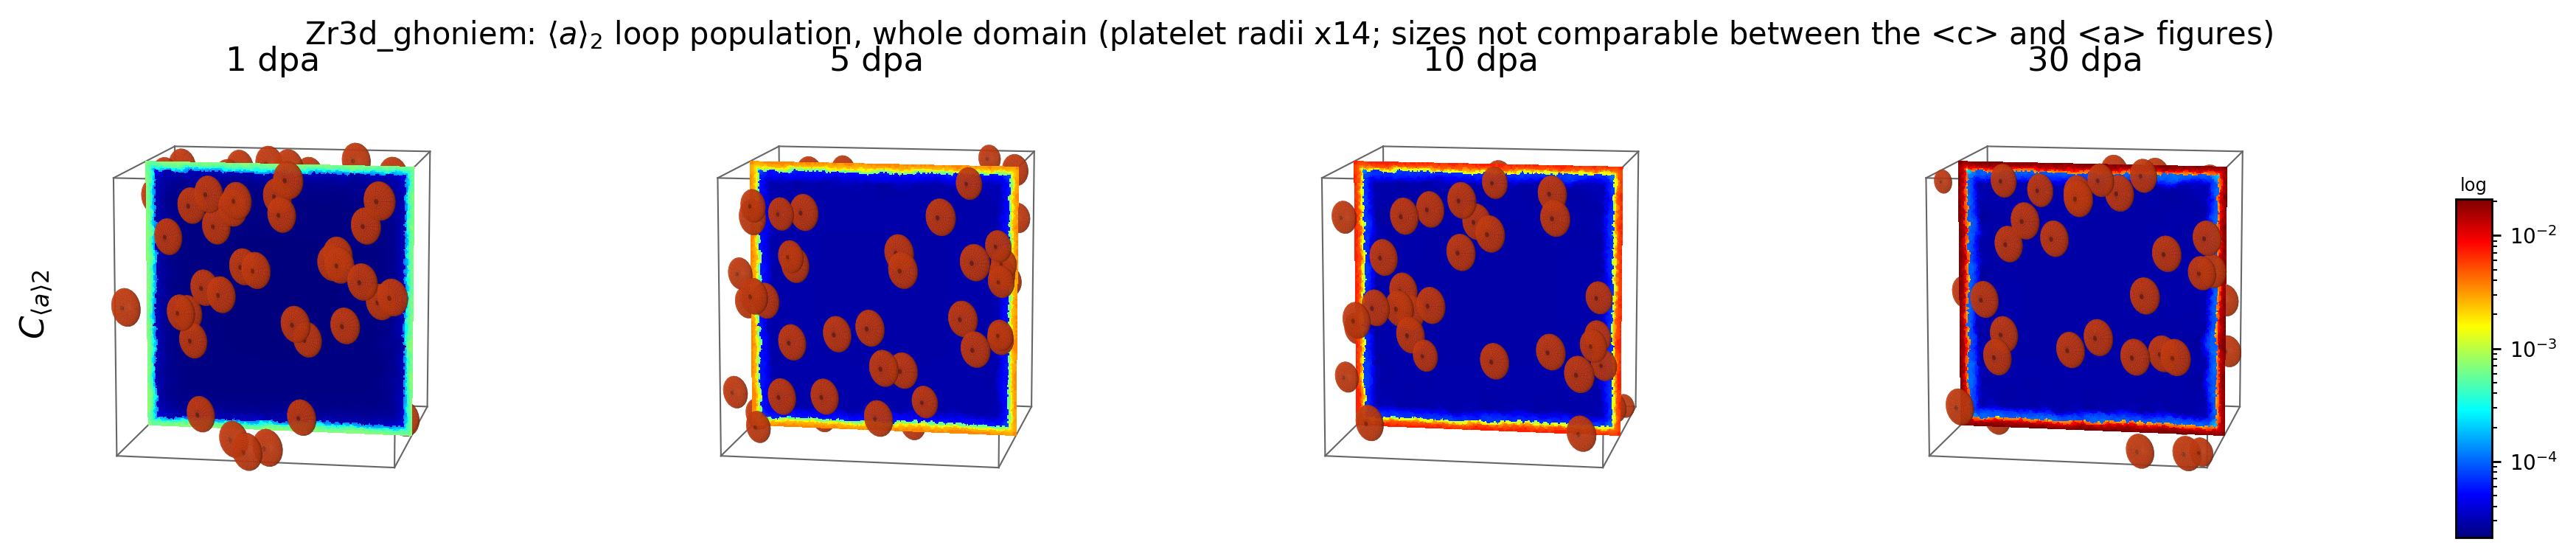
\includegraphics[width=0.85\linewidth,height=0.72\textheight,keepaspectratio]{figures/loops_a2_overlay.png}\\[4pt]
\footnotesize Second $\langle a\rangle$-loop family $C_{(a)2}$ on the same domain and dose sequence; the growing number and size of markers track progressive $\langle a\rangle$-loop accumulation.
\end{frame}

\begin{frame}{$\langle a\rangle$-loop population: family~3}
\centering
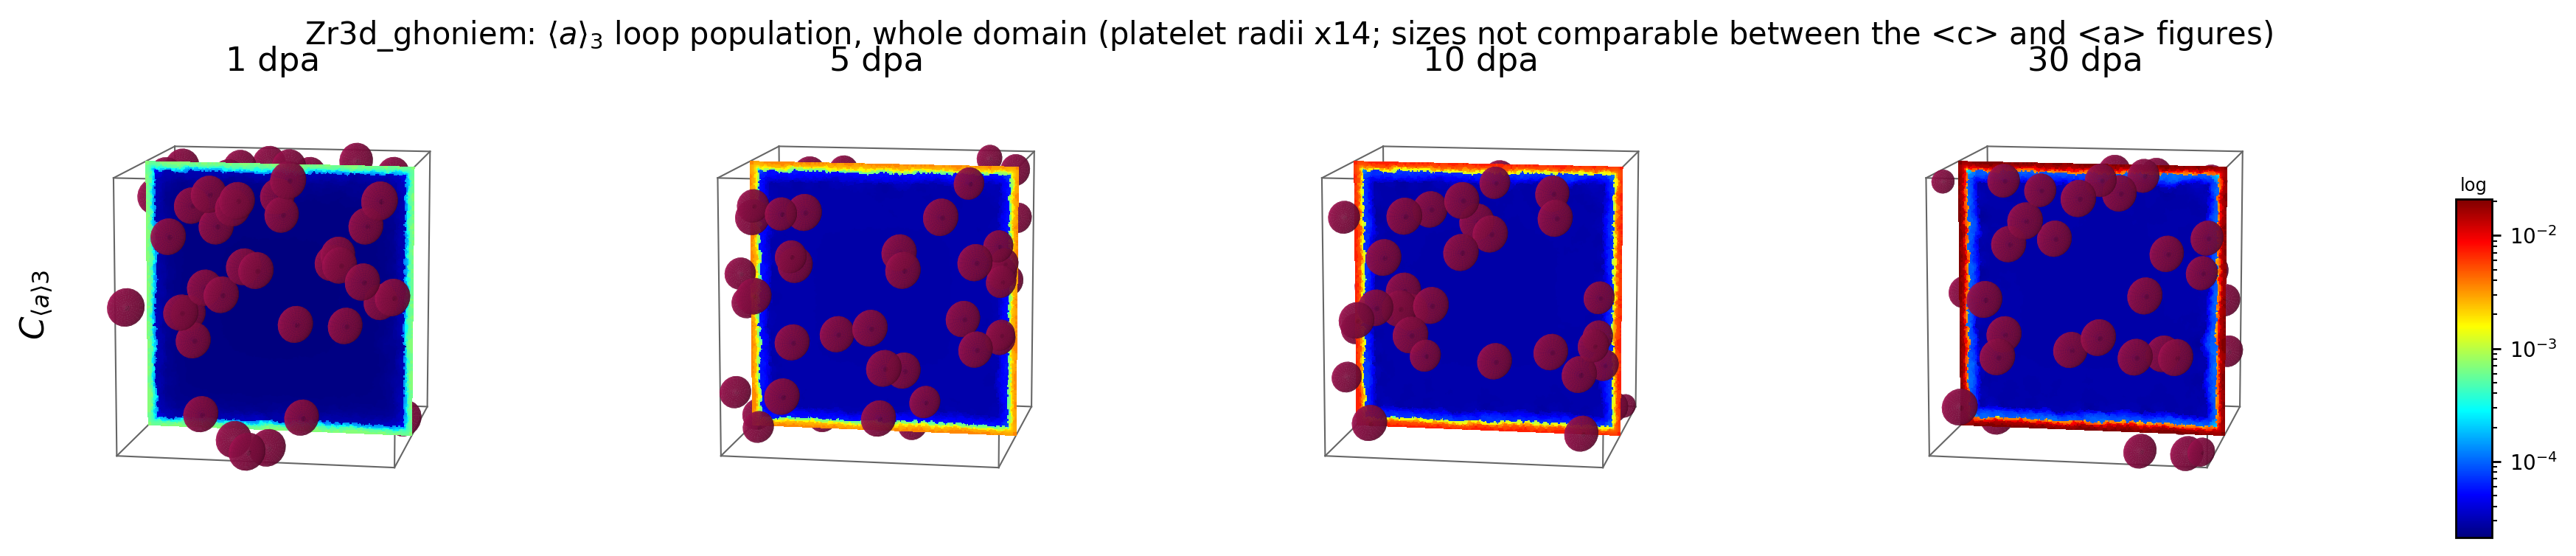
\includegraphics[width=0.85\linewidth,height=0.72\textheight,keepaspectratio]{figures/loops_a3_overlay.png}\\[4pt]
\footnotesize Third $\langle a\rangle$-loop family $C_{(a)3}$; together the three families represent the full $\langle a\rangle$-type interstitial loop distribution that feeds the dislocation network.
\end{frame}

\begin{frame}{$\langle c\rangle$-loop population}
\centering
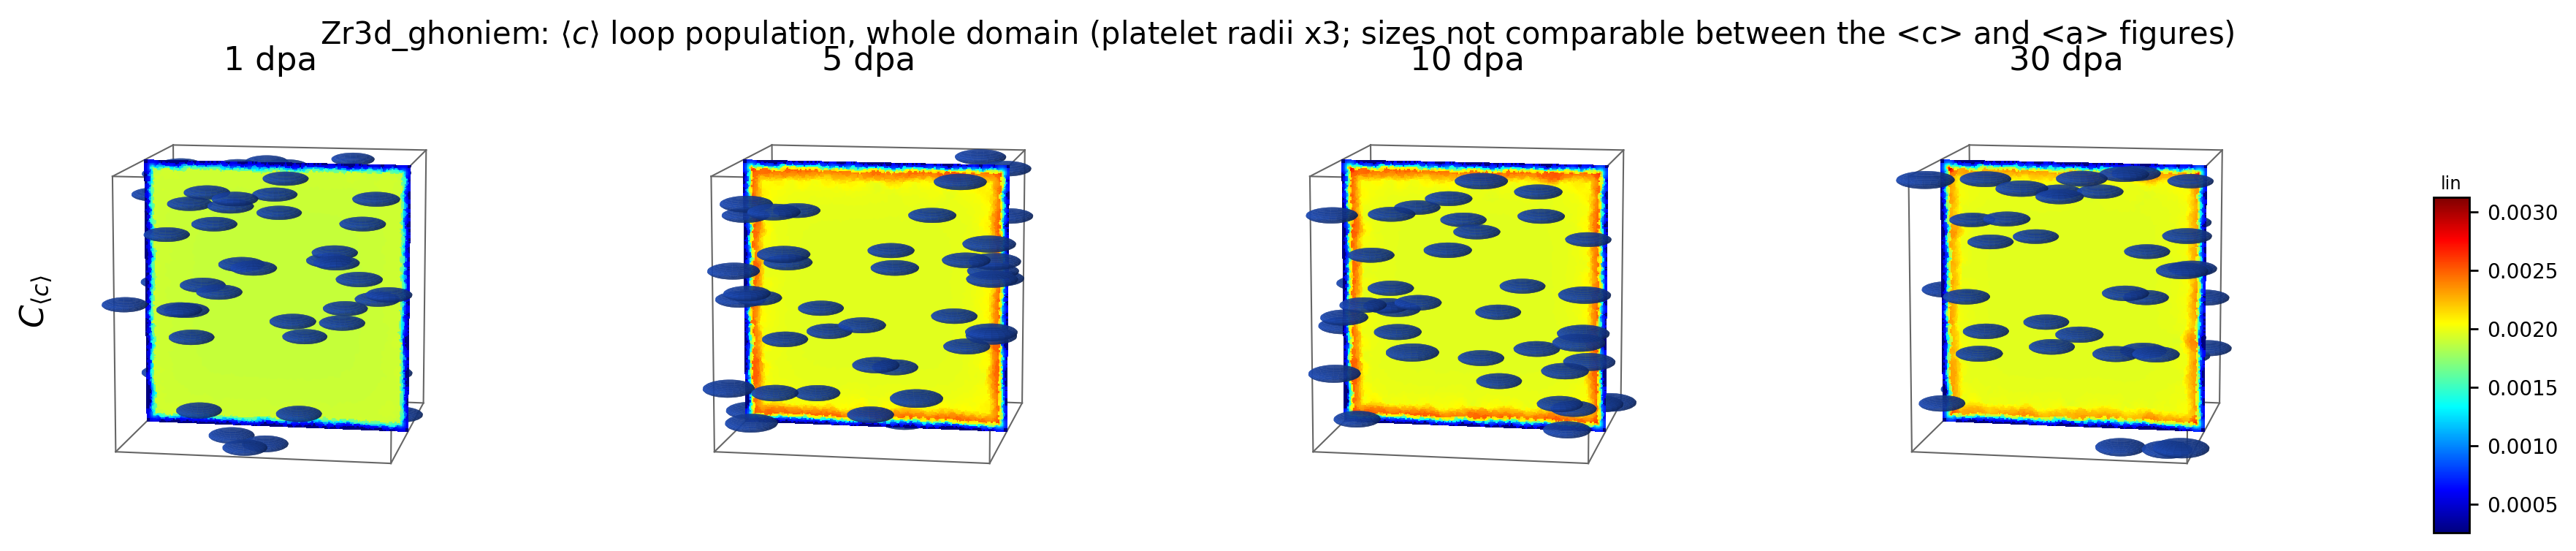
\includegraphics[width=0.85\linewidth,height=0.72\textheight,keepaspectratio]{figures/loops_c_overlay.png}\\[4pt]
\footnotesize Vacancy $\langle c\rangle$-loop population $C_{(c)}$ over the domain at $1$--$30\,$dpa (linear colour scale, platelet markers $\times3$). The $\langle c\rangle$-loops are fewer but individually larger than the $\langle a\rangle$-loops; marker sizes are not comparable between the $\langle c\rangle$ and $\langle a\rangle$ figures.
\end{frame}

\begin{frame}{Dislocation-loop number density vs.\ dose}
\centering
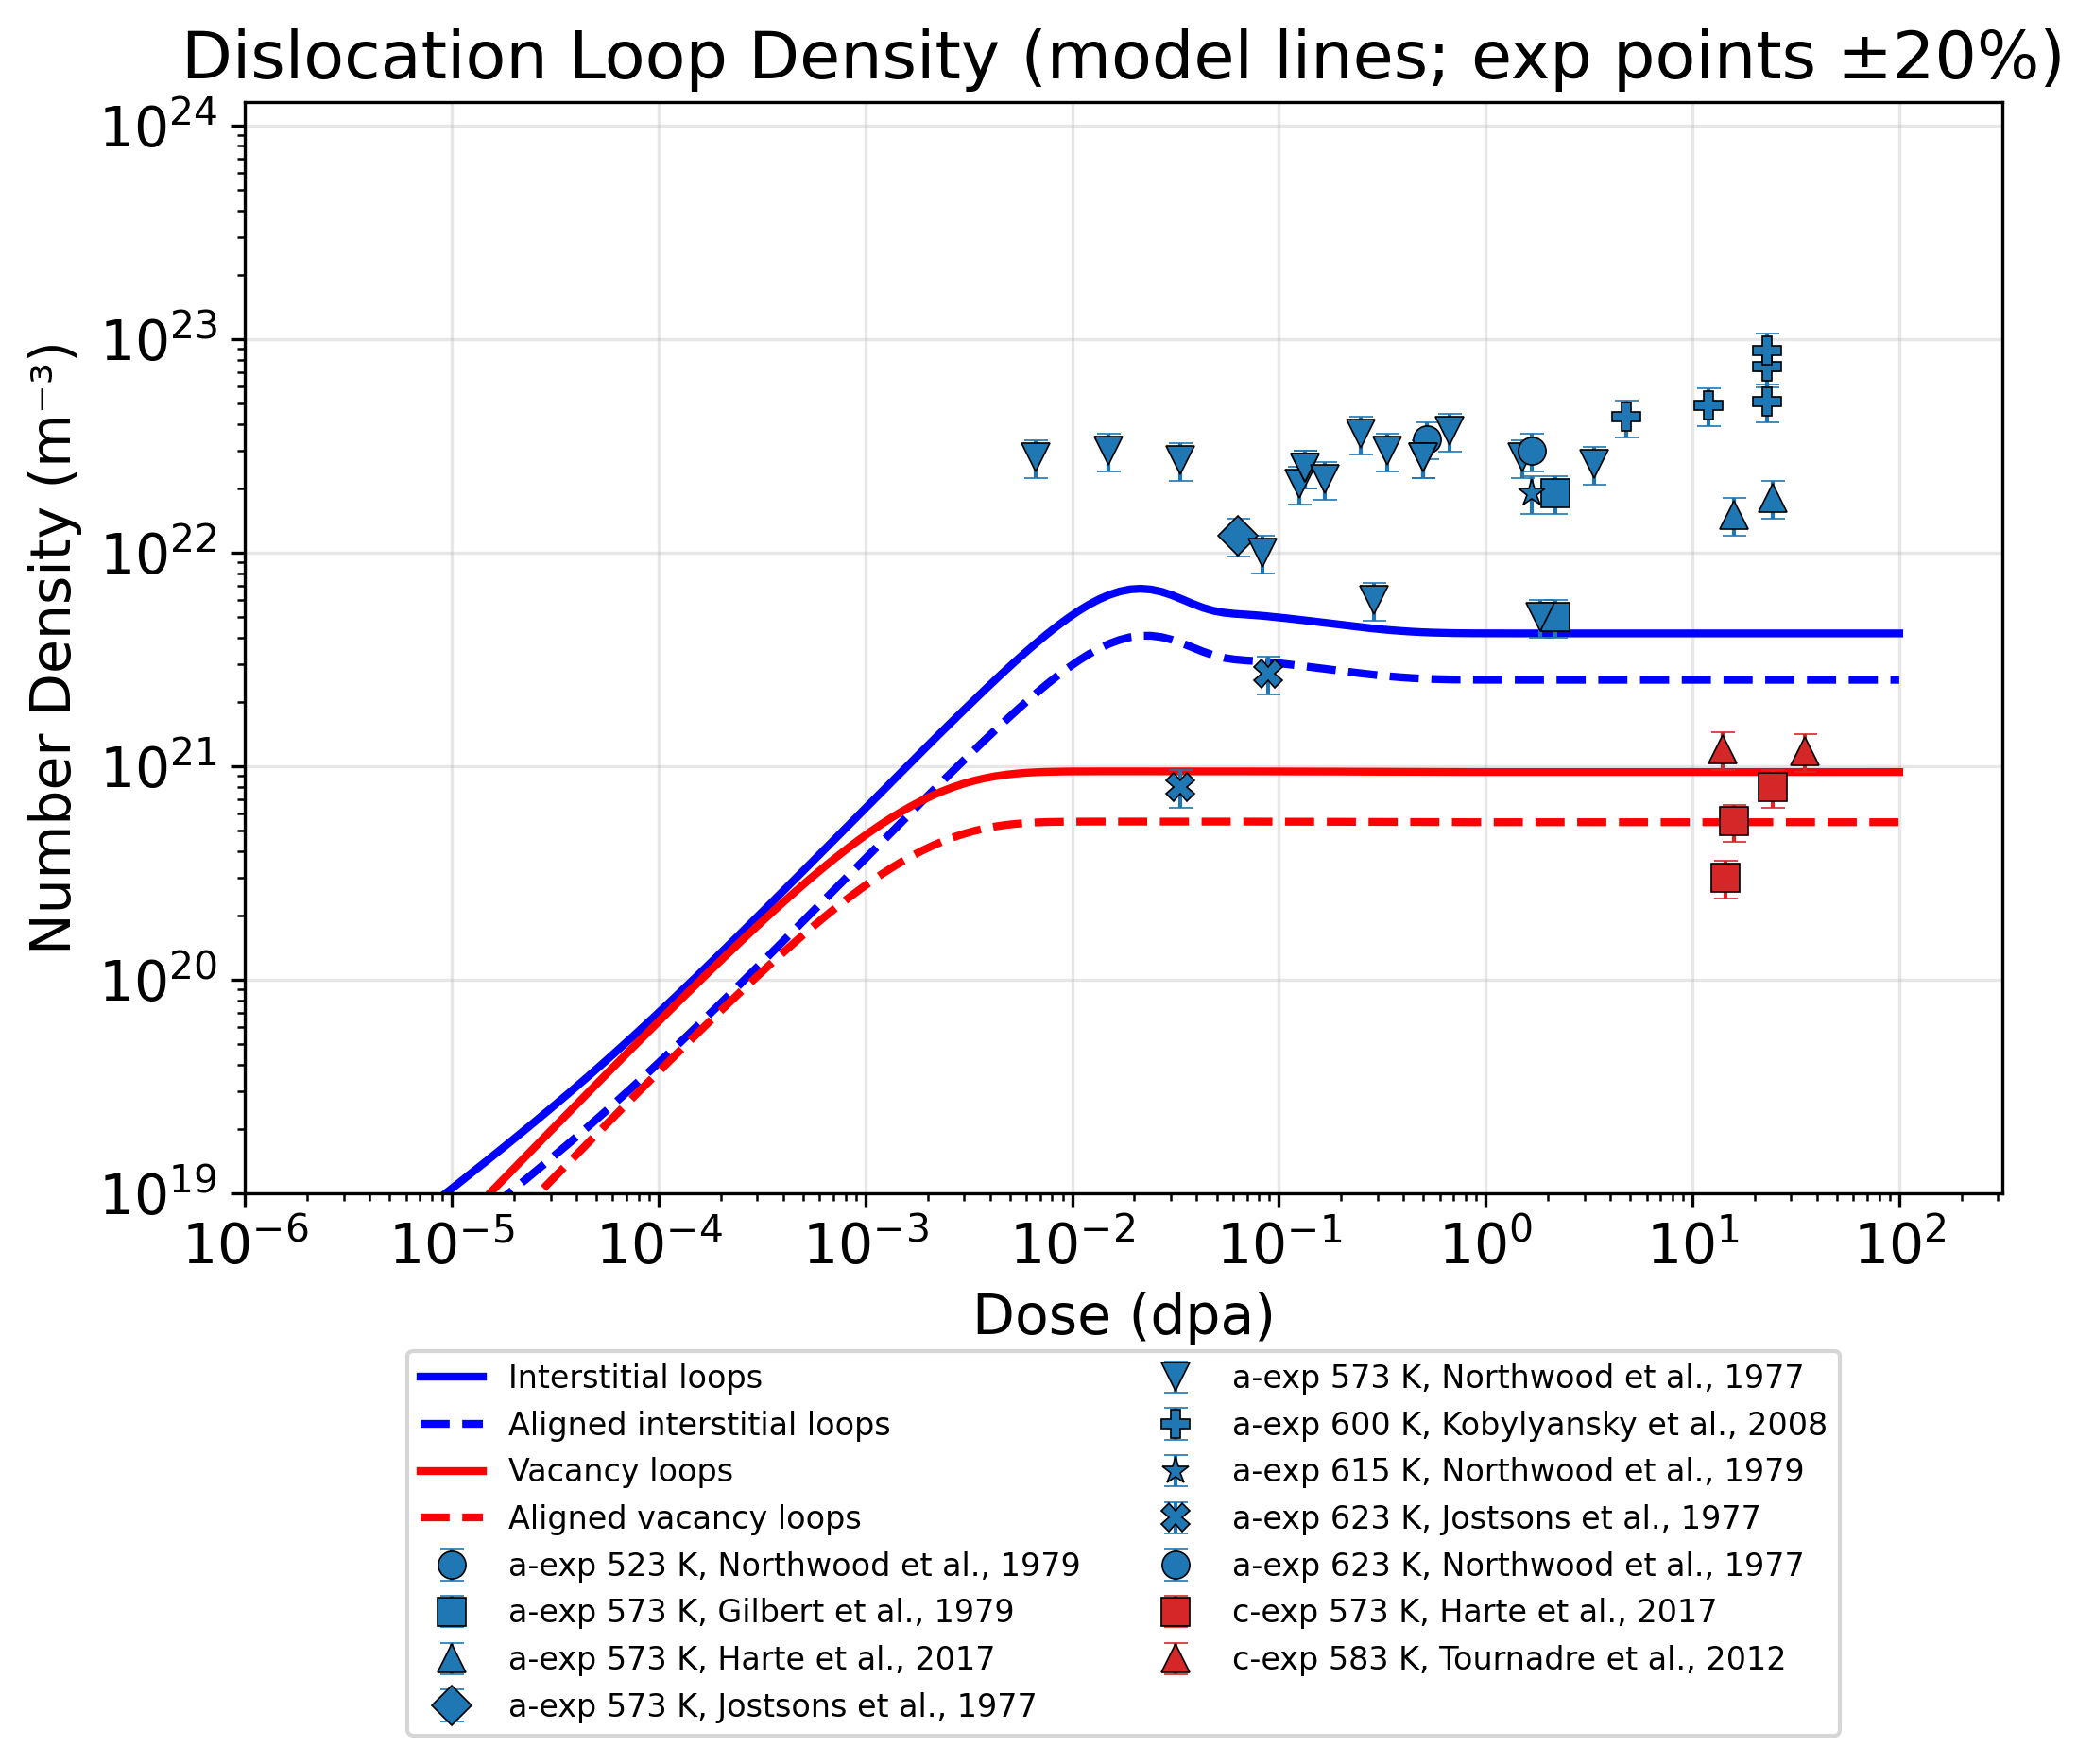
\includegraphics[width=0.85\linewidth,height=0.72\textheight,keepaspectratio]{figures/loop_density.png}\\[4pt]
\footnotesize Model loop number densities (interstitial and vacancy, total and network-aligned) compared with the experimental Zr database ($\pm20\%$). Interstitial $\langle a\rangle$-loops saturate near a few $\times10^{21}\,\mathrm{m^{-3}}$ and vacancy loops near $10^{21}\,\mathrm{m^{-3}}$.
\end{frame}

\begin{frame}{Loop diameter vs.\ dose}
\centering
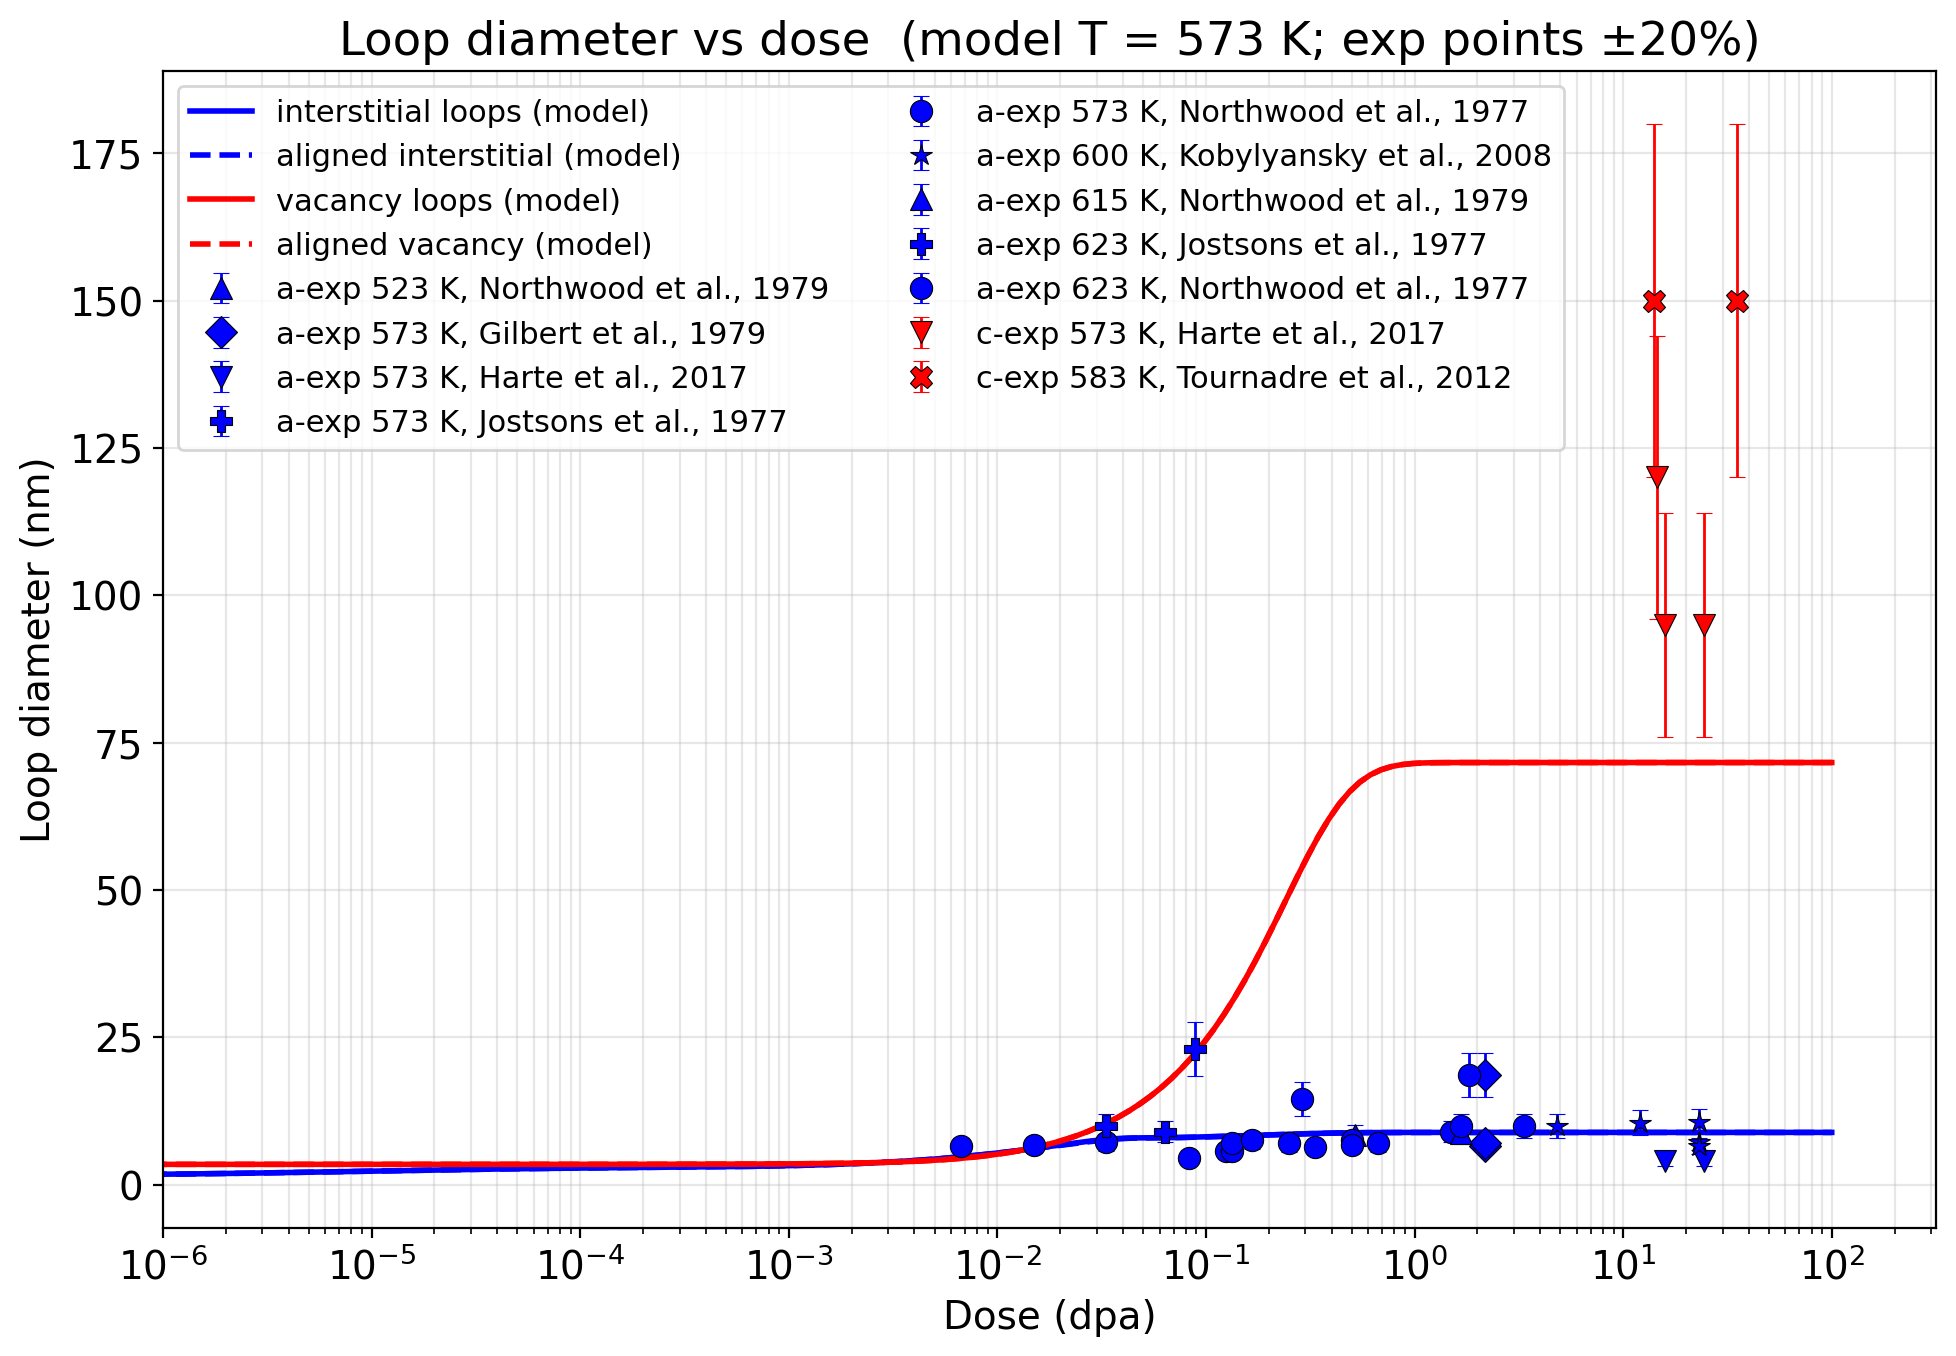
\includegraphics[width=0.85\linewidth,height=0.72\textheight,keepaspectratio]{figures/loop_diameter_vs_dose.png}\\[4pt]
\footnotesize Predicted mean loop diameters at $T=573\,$K against experiment ($\pm20\%$). Interstitial loops plateau near $9$--$10\,$nm, while vacancy $\langle c\rangle$-loops grow past $\sim\!10^{-1}\,$dpa toward $\sim\!70\,$nm.
\end{frame}

\begin{frame}{Loop--network spacing vs.\ dose}
\centering
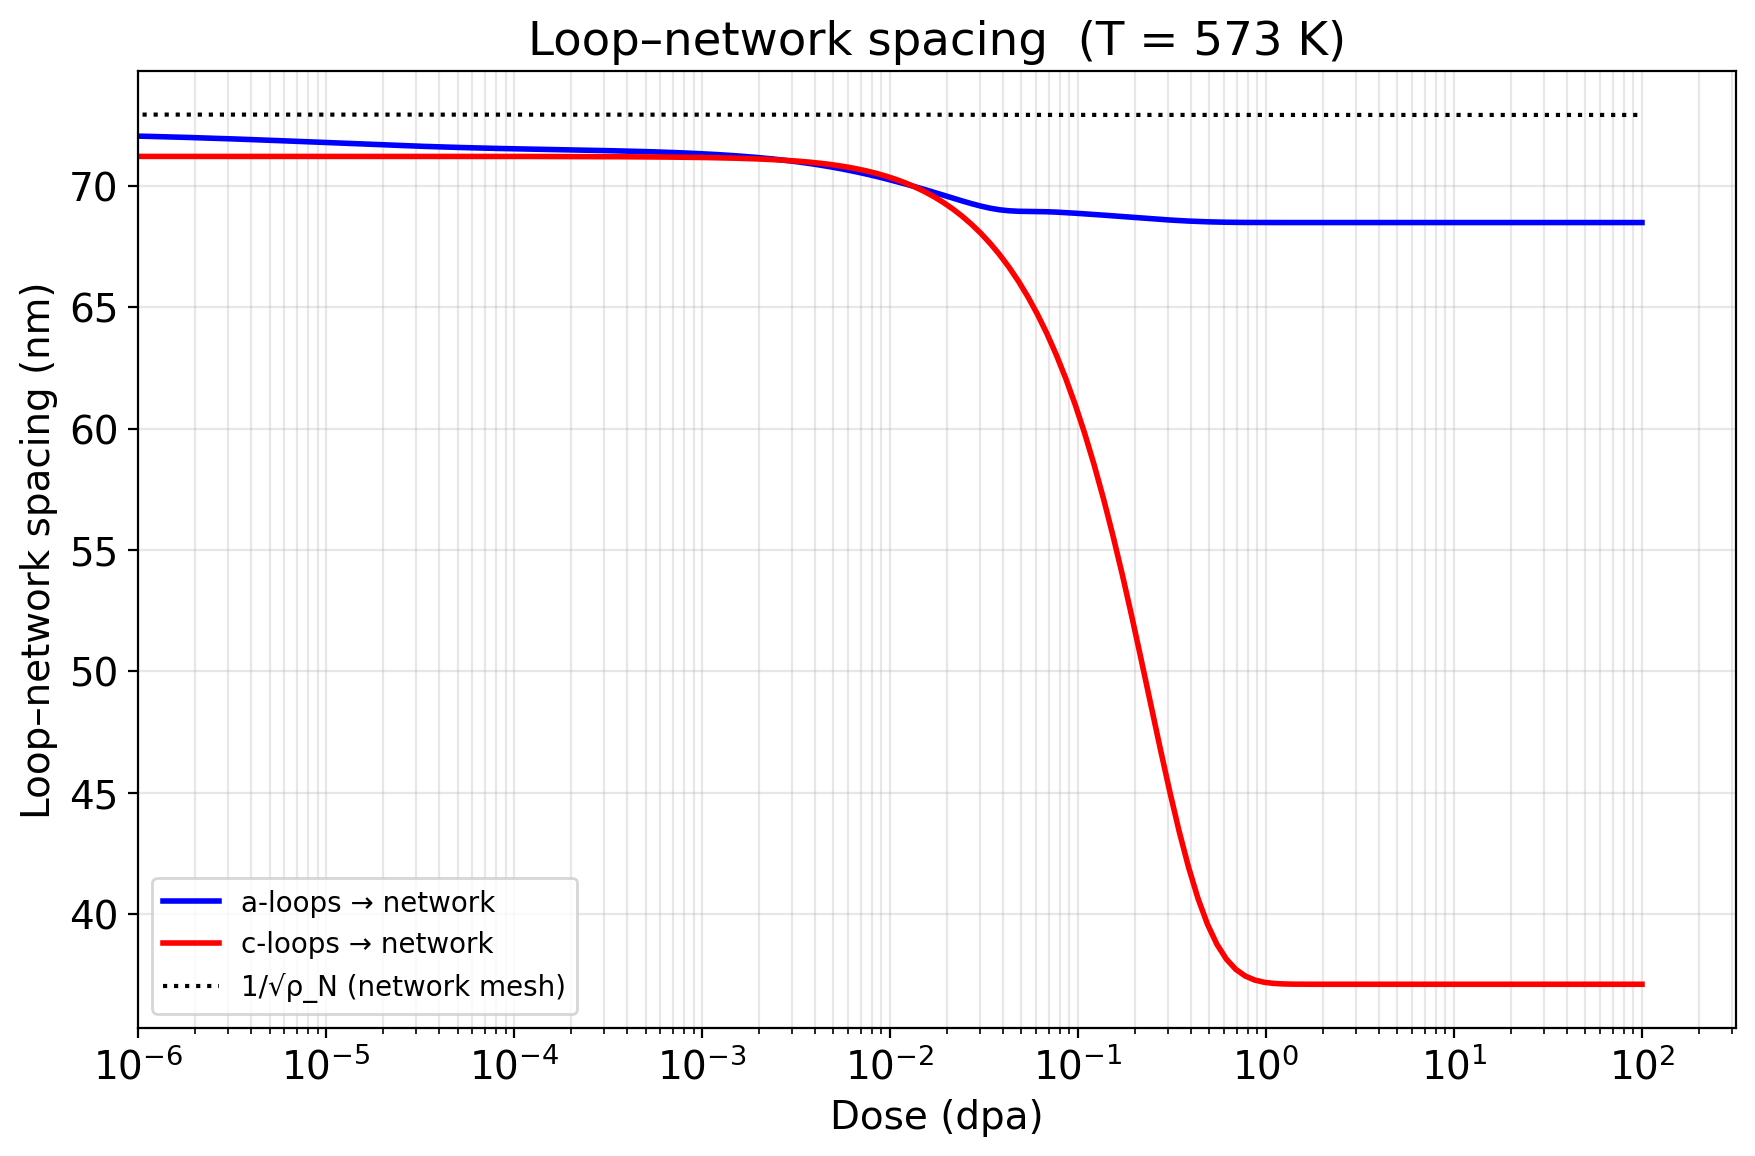
\includegraphics[width=0.85\linewidth,height=0.72\textheight,keepaspectratio]{figures/loop_network_spacing.png}\\[4pt]
\footnotesize The mean spacing between loops and the dislocation network. The $\langle a\rangle$-loop spacing stays close to the network mesh size of $1/\sqrt{\rho_N}\approx70\,$nm, whereas the $\langle c\rangle$-loop spacing collapses to $\sim\!37\,$nm above $\sim\!1\,$dpa as the $\langle c\rangle$-loops densify.
\end{frame}

\begin{frame}{Grain boundary content profiles}
\centering
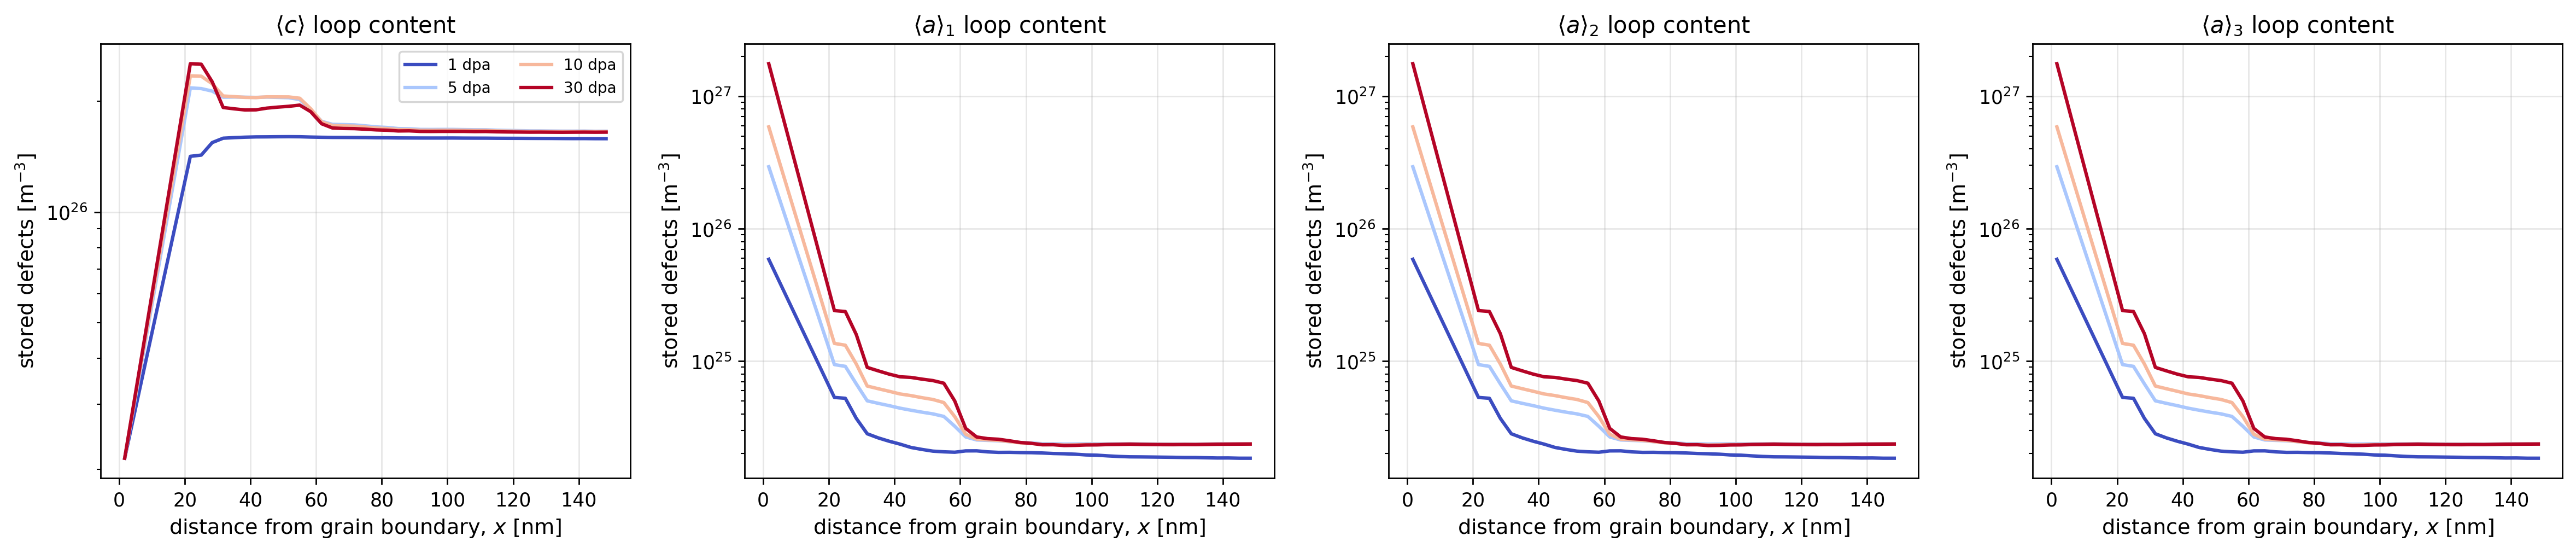
\includegraphics[width=0.85\linewidth,height=0.72\textheight,keepaspectratio]{figures/gb_content_profiles.png}\\[4pt]
\footnotesize The mean spacing between loops and the dislocation network. The $\langle a\rangle$-loop spacing stays close to the network mesh size of $1/\sqrt{\rho_N}\approx70\,$nm, whereas the $\langle c\rangle$-loop spacing collapses to $\sim\!37\,$nm above $\sim\!1\,$dpa as the $\langle c\rangle$-loops densify.
\end{frame}

\begin{frame}{Grain boundary density profiles}
\centering
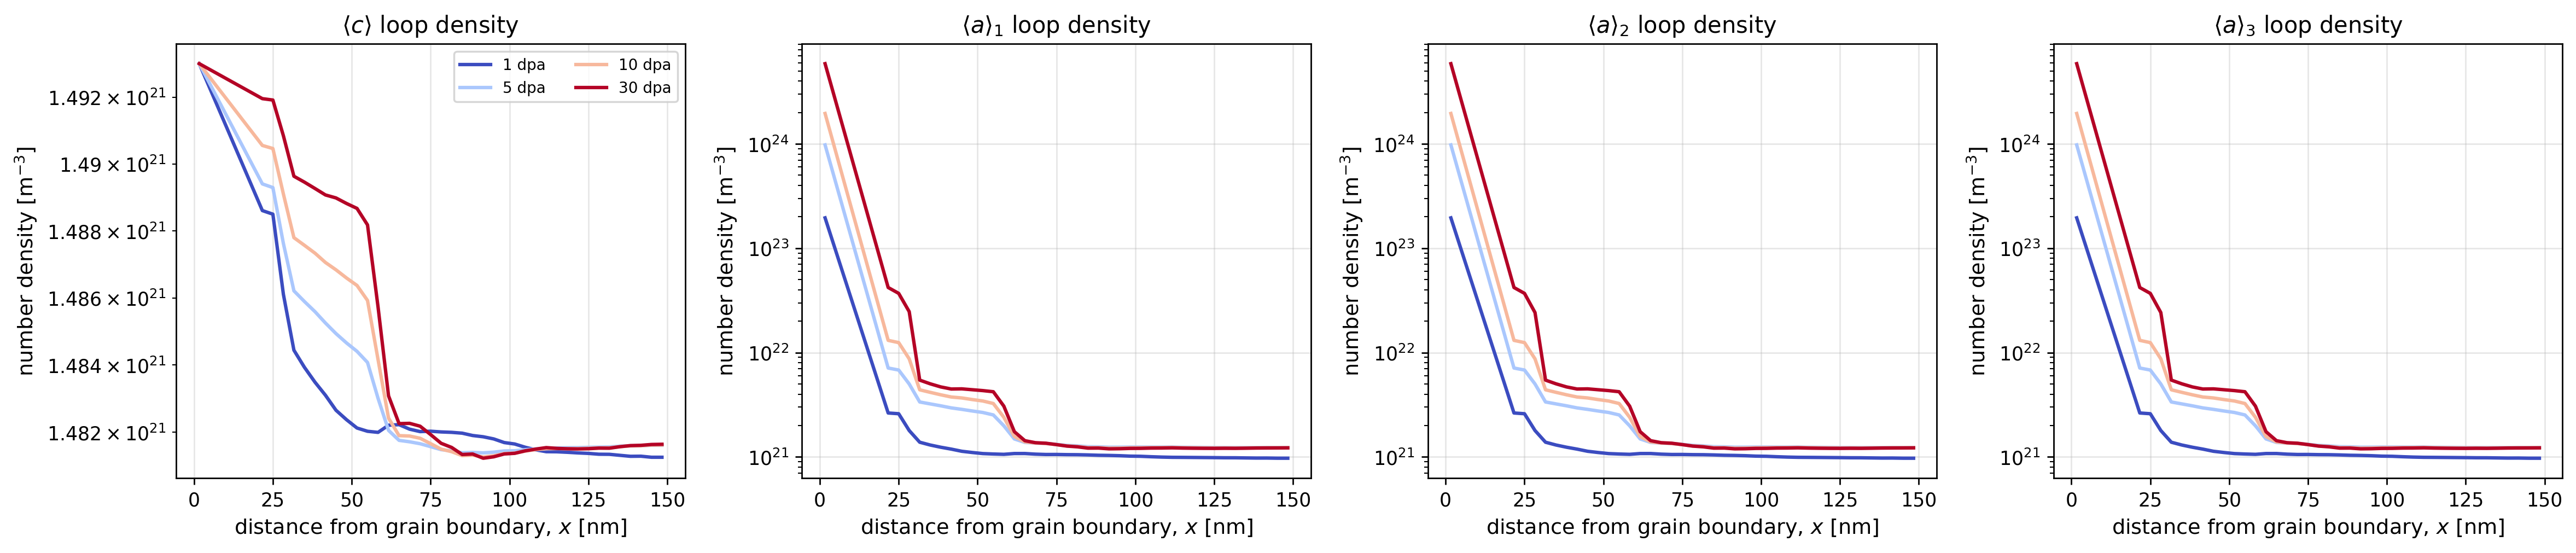
\includegraphics[width=0.85\linewidth,height=0.72\textheight,keepaspectratio]{figures/gb_density_profiles.png}\\[4pt]
\footnotesize The mean spacing between loops and the dislocation network. The $\langle a\rangle$-loop spacing stays close to the network mesh size of $1/\sqrt{\rho_N}\approx70\,$nm, whereas the $\langle c\rangle$-loop spacing collapses to $\sim\!37\,$nm above $\sim\!1\,$dpa as the $\langle c\rangle$-loops densify.
\end{frame}

\begin{frame}{Grain boundary mobile profiles}
\centering
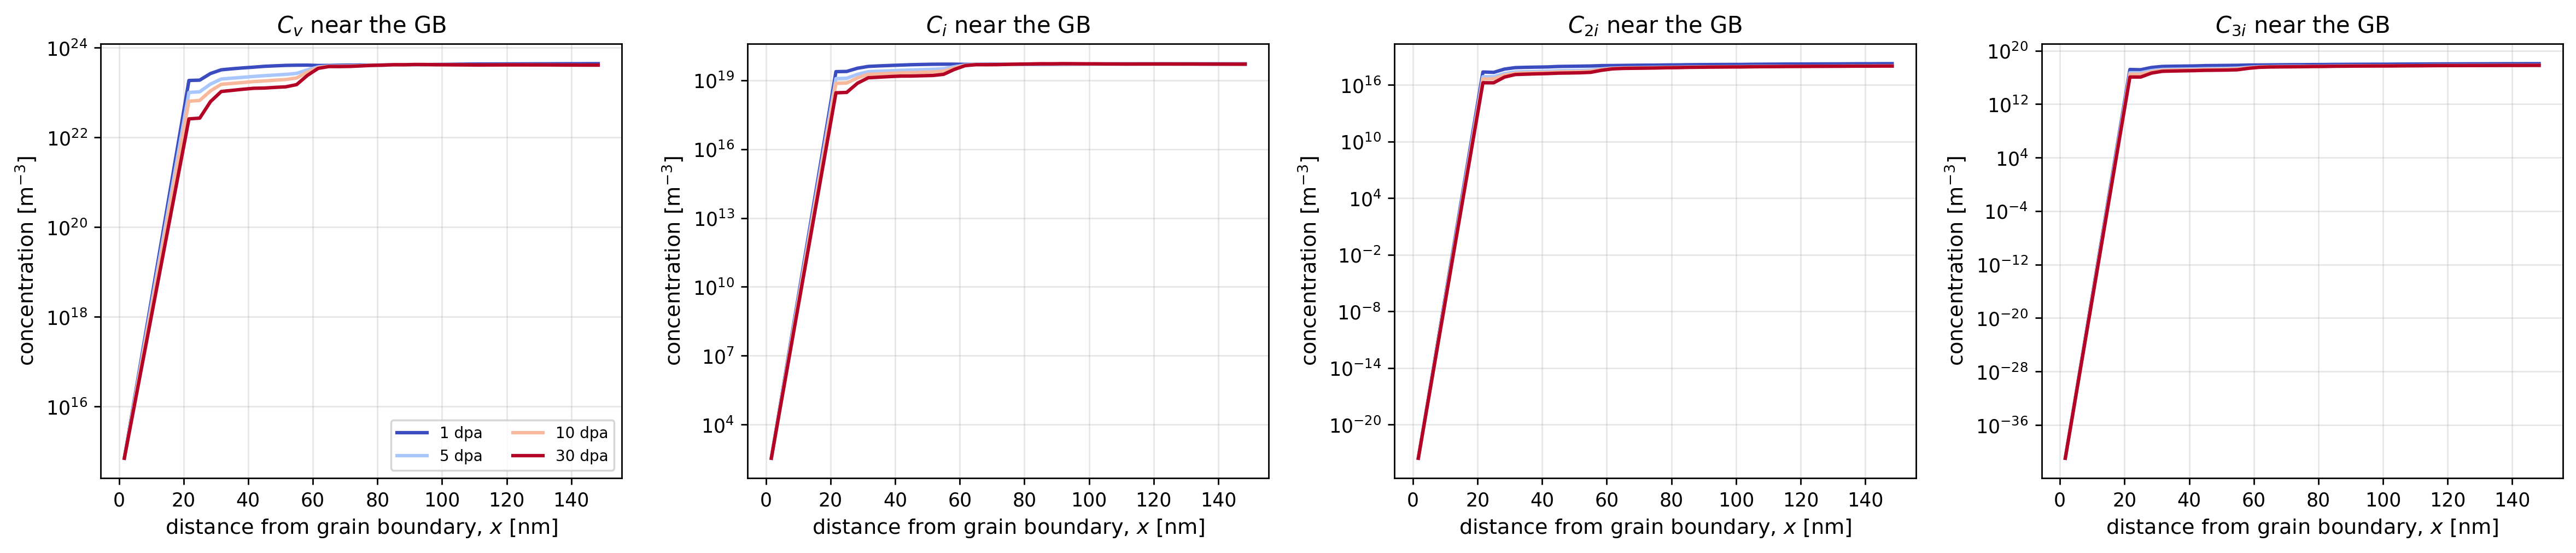
\includegraphics[width=0.85\linewidth,height=0.72\textheight,keepaspectratio]{figures/gb_mobile_profiles.png}\\[4pt]
\footnotesize The mean spacing between loops and the dislocation network. The $\langle a\rangle$-loop spacing stays close to the network mesh size of $1/\sqrt{\rho_N}\approx70\,$nm, whereas the $\langle c\rangle$-loop spacing collapses to $\sim\!37\,$nm above $\sim\!1\,$dpa as the $\langle c\rangle$-loops densify.
\end{frame}

\begin{frame}{Grain boundary size profiles}
\centering
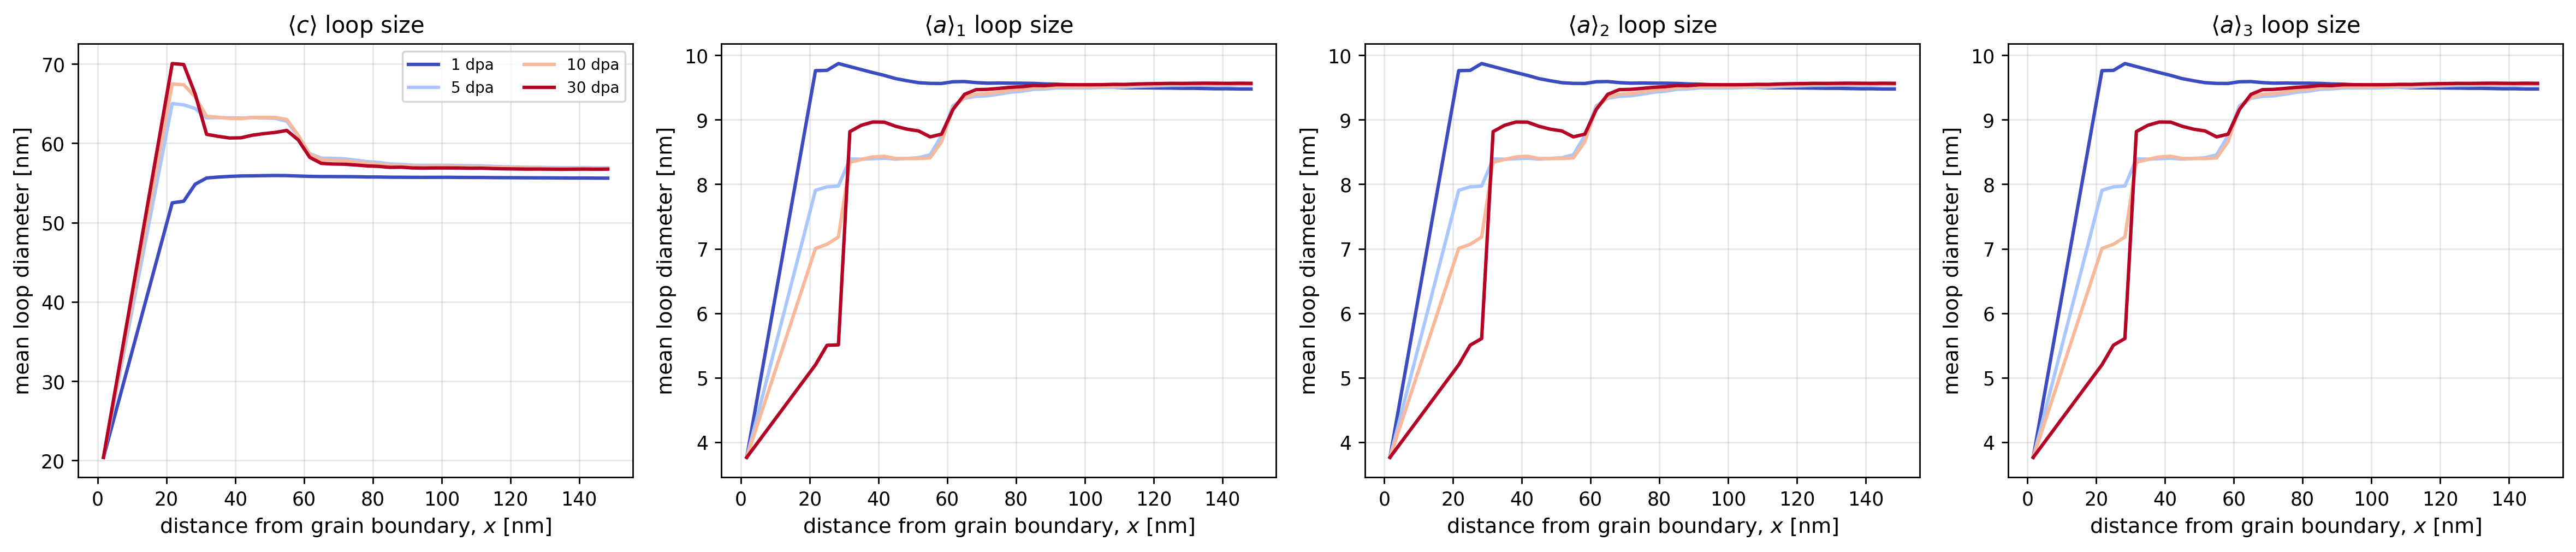
\includegraphics[width=0.85\linewidth,height=0.72\textheight,keepaspectratio]{figures/gb_size_profiles.png}\\[4pt]
\footnotesize The mean spacing between loops and the dislocation network. The $\langle a\rangle$-loop spacing stays close to the network mesh size of $1/\sqrt{\rho_N}\approx70\,$nm, whereas the $\langle c\rangle$-loop spacing collapses to $\sim\!37\,$nm above $\sim\!1\,$dpa as the $\langle c\rangle$-loops densify.
\end{frame}

\begin{frame}{Mesh Dependence Studies}
\centering
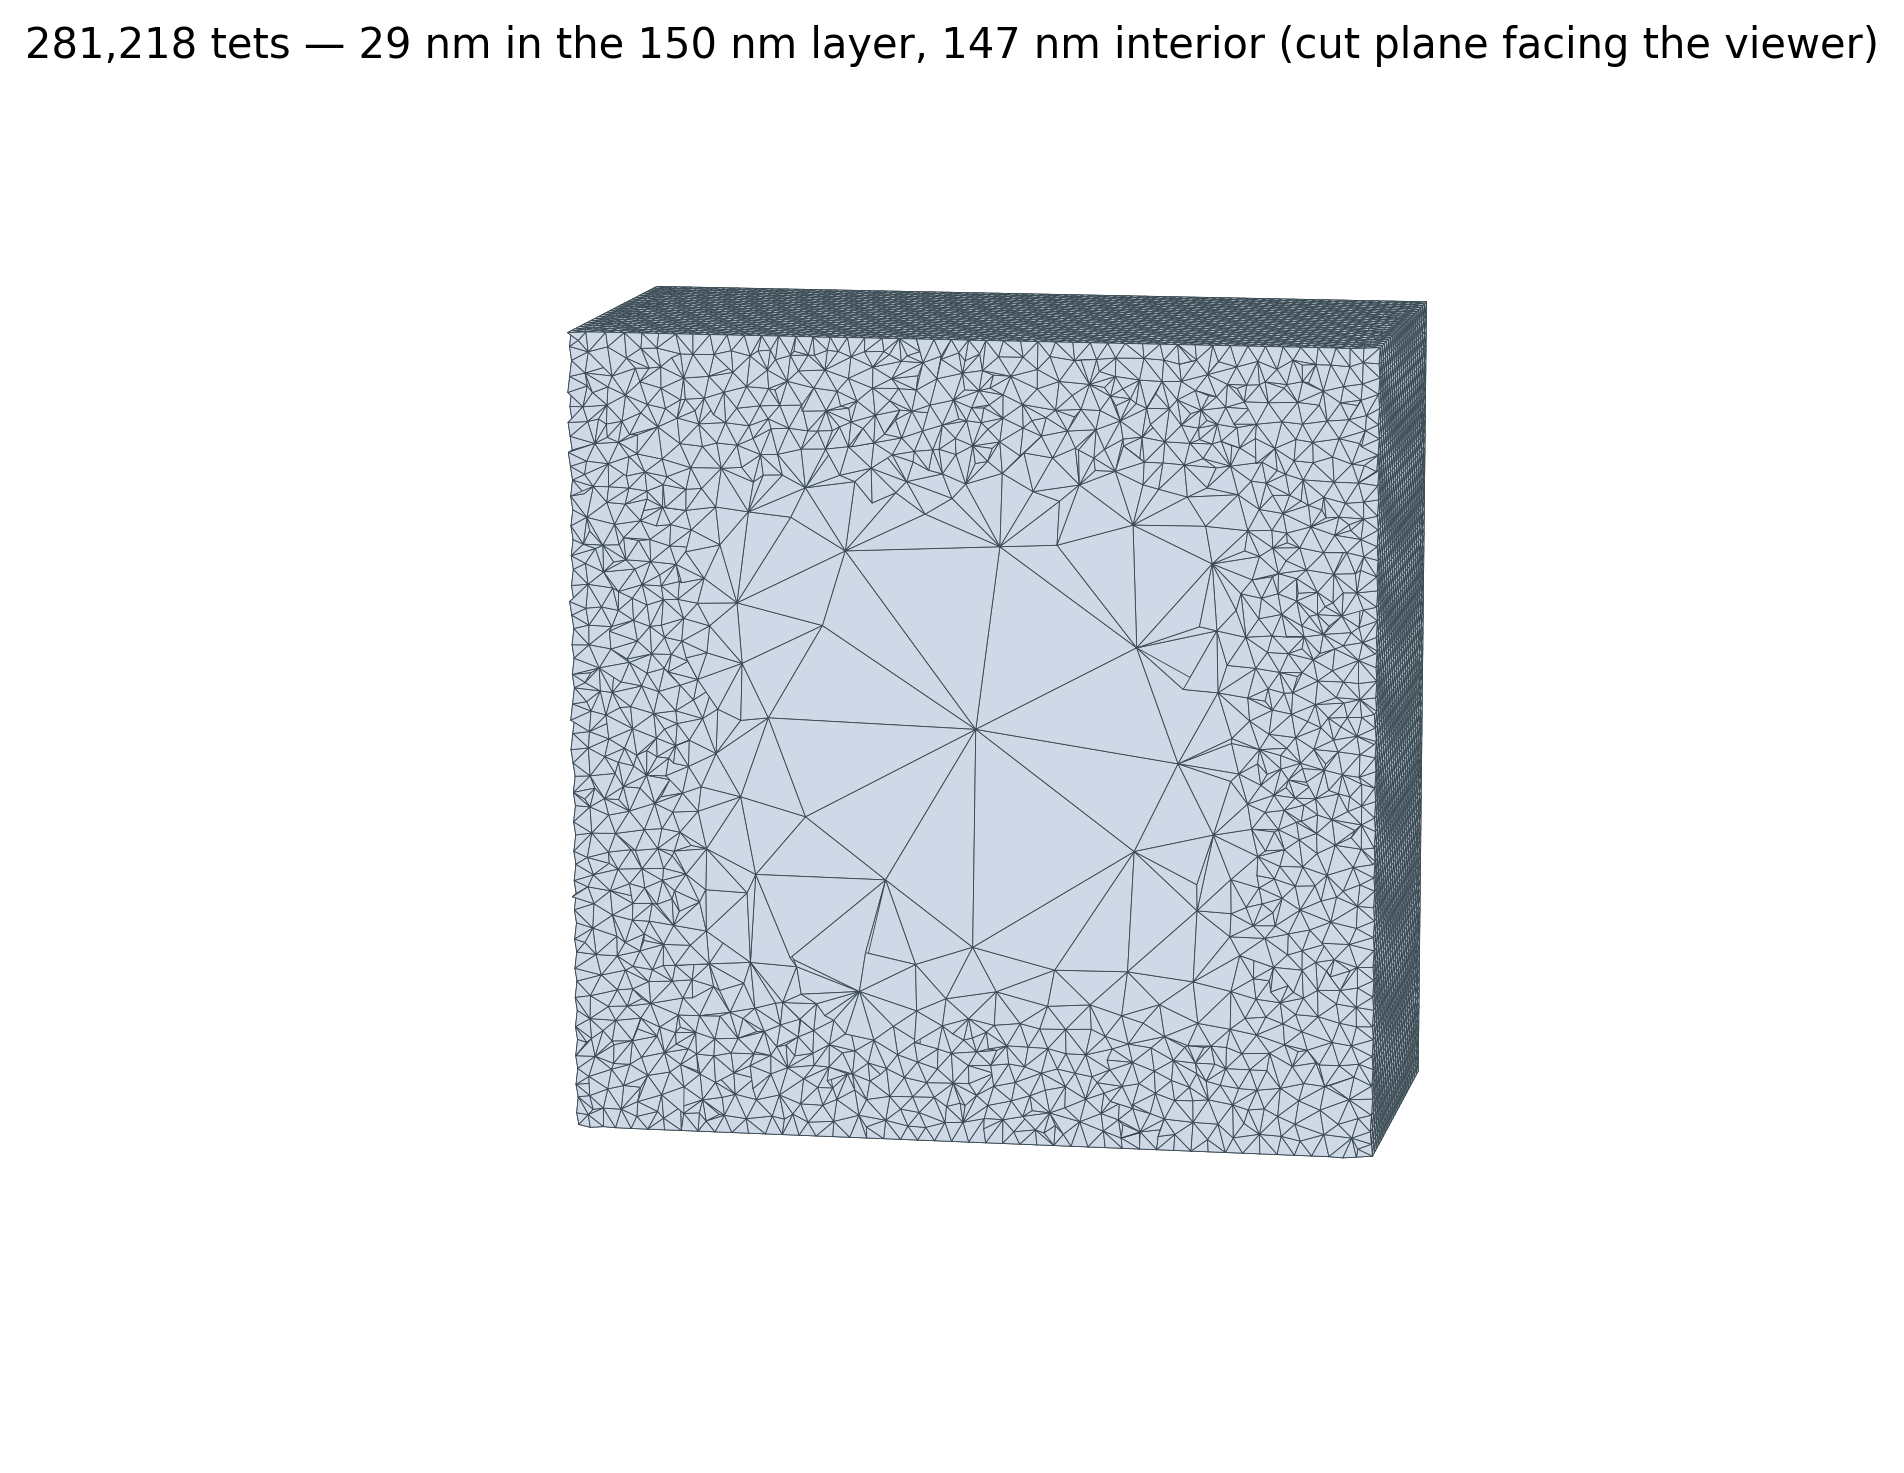
\includegraphics[width=0.45\linewidth]{figures/mesh_E_281218tets.png}
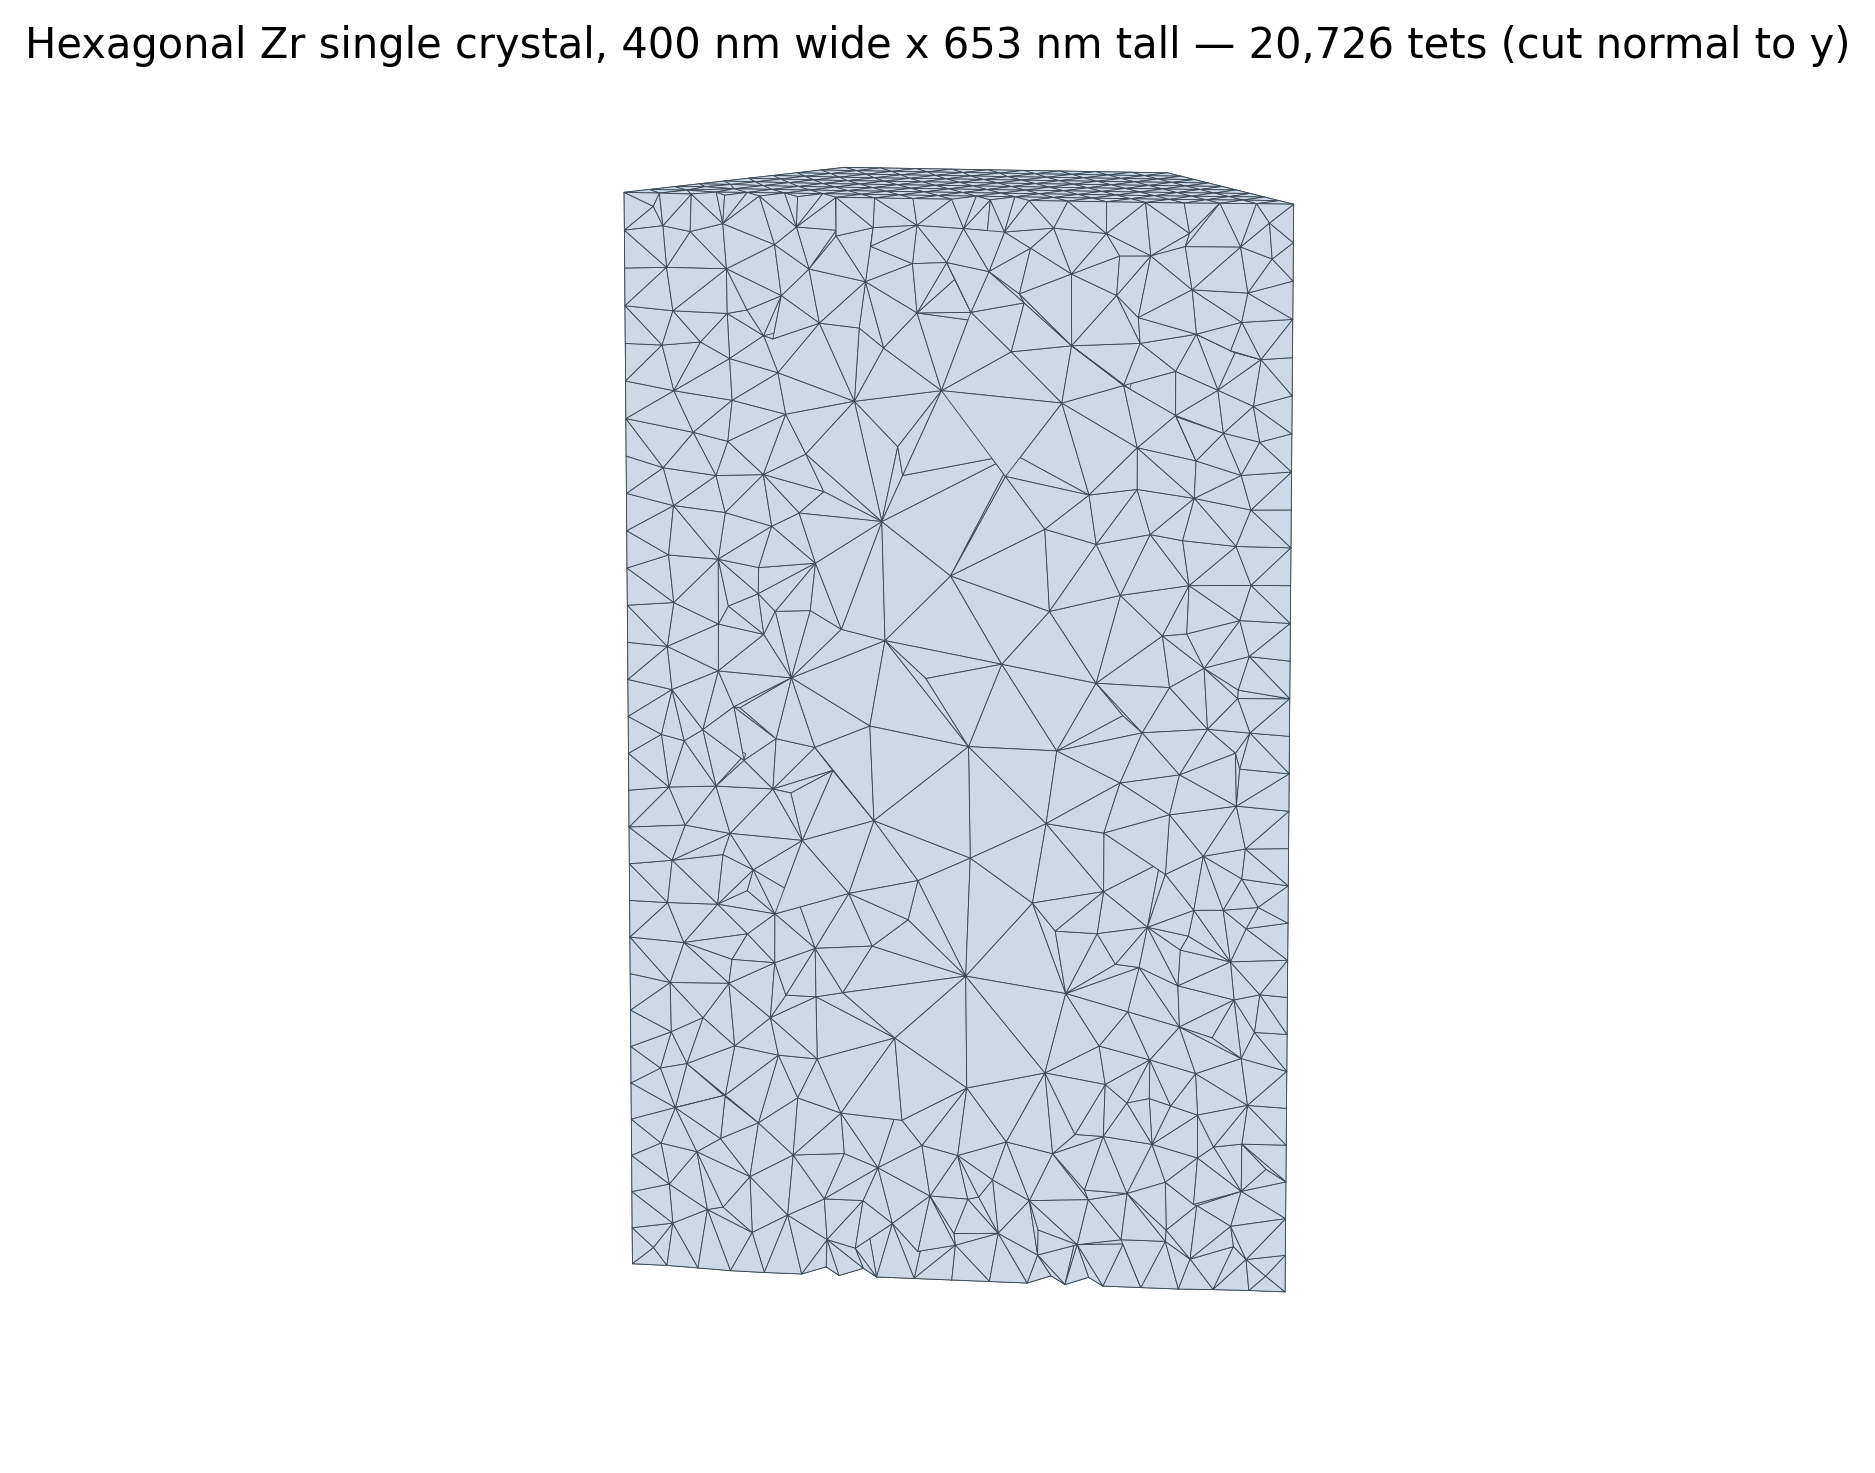
\includegraphics[width=0.45\linewidth]{figures/mesh_hex400_cut_y.png}
\end{frame}

\begin{frame}{a-Loop Size Distributions}
\centering
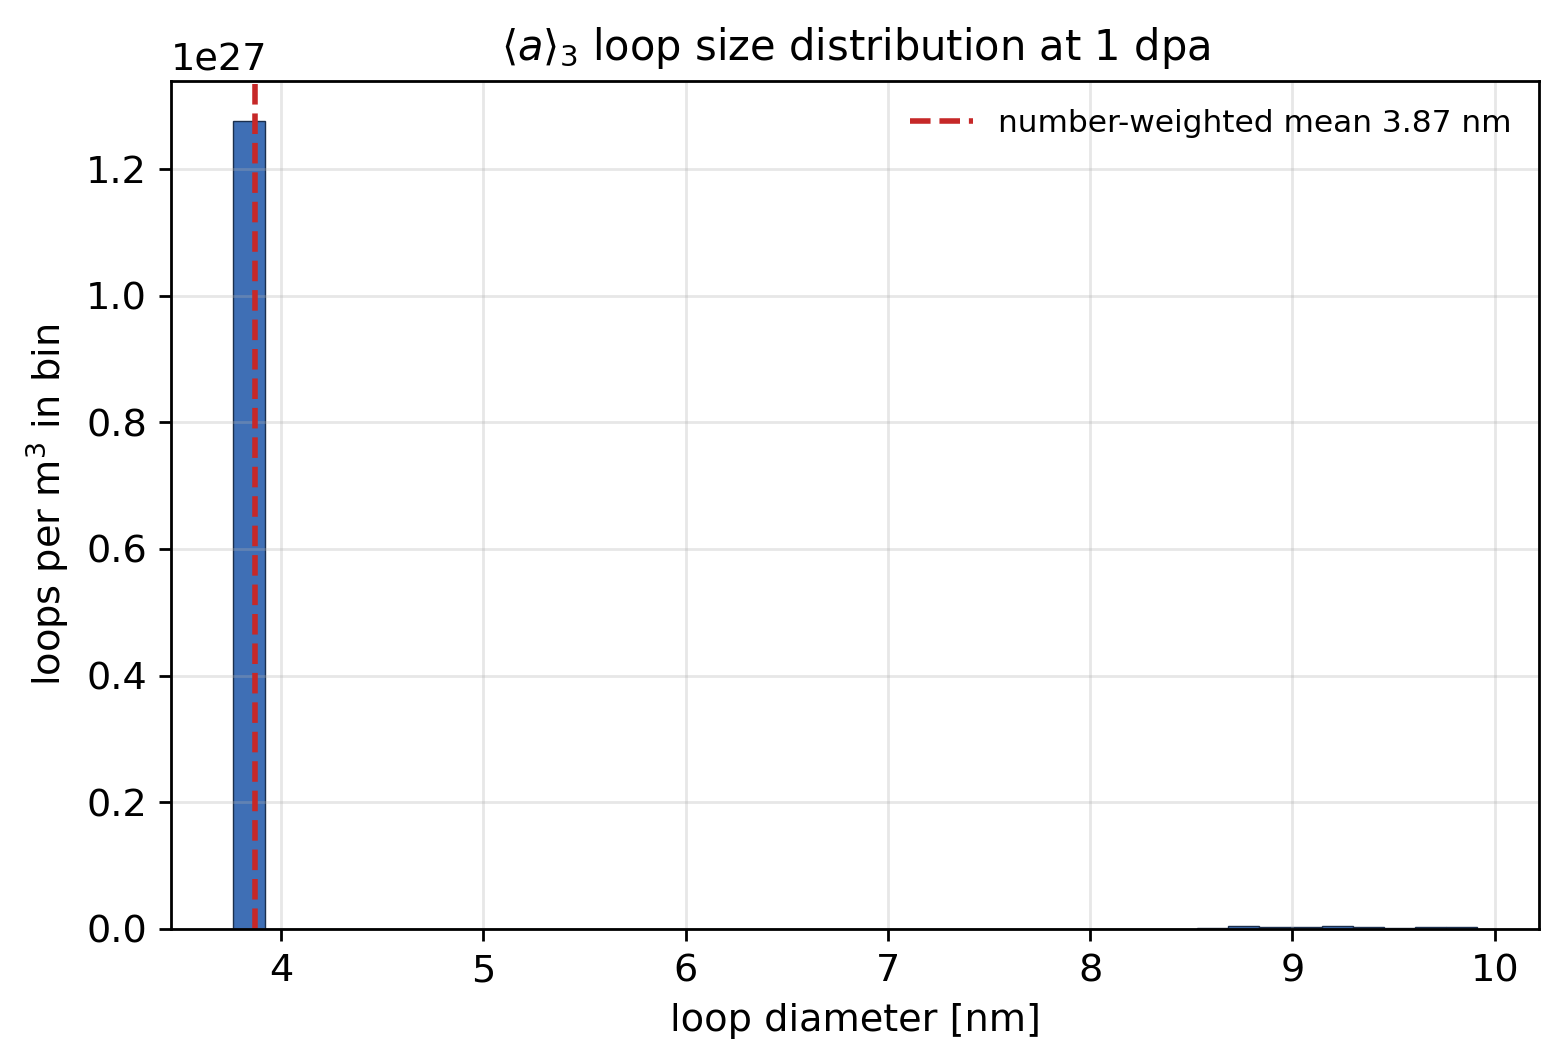
\includegraphics[width=0.45\linewidth]{figures/size_dist_a3_01dpa.png}
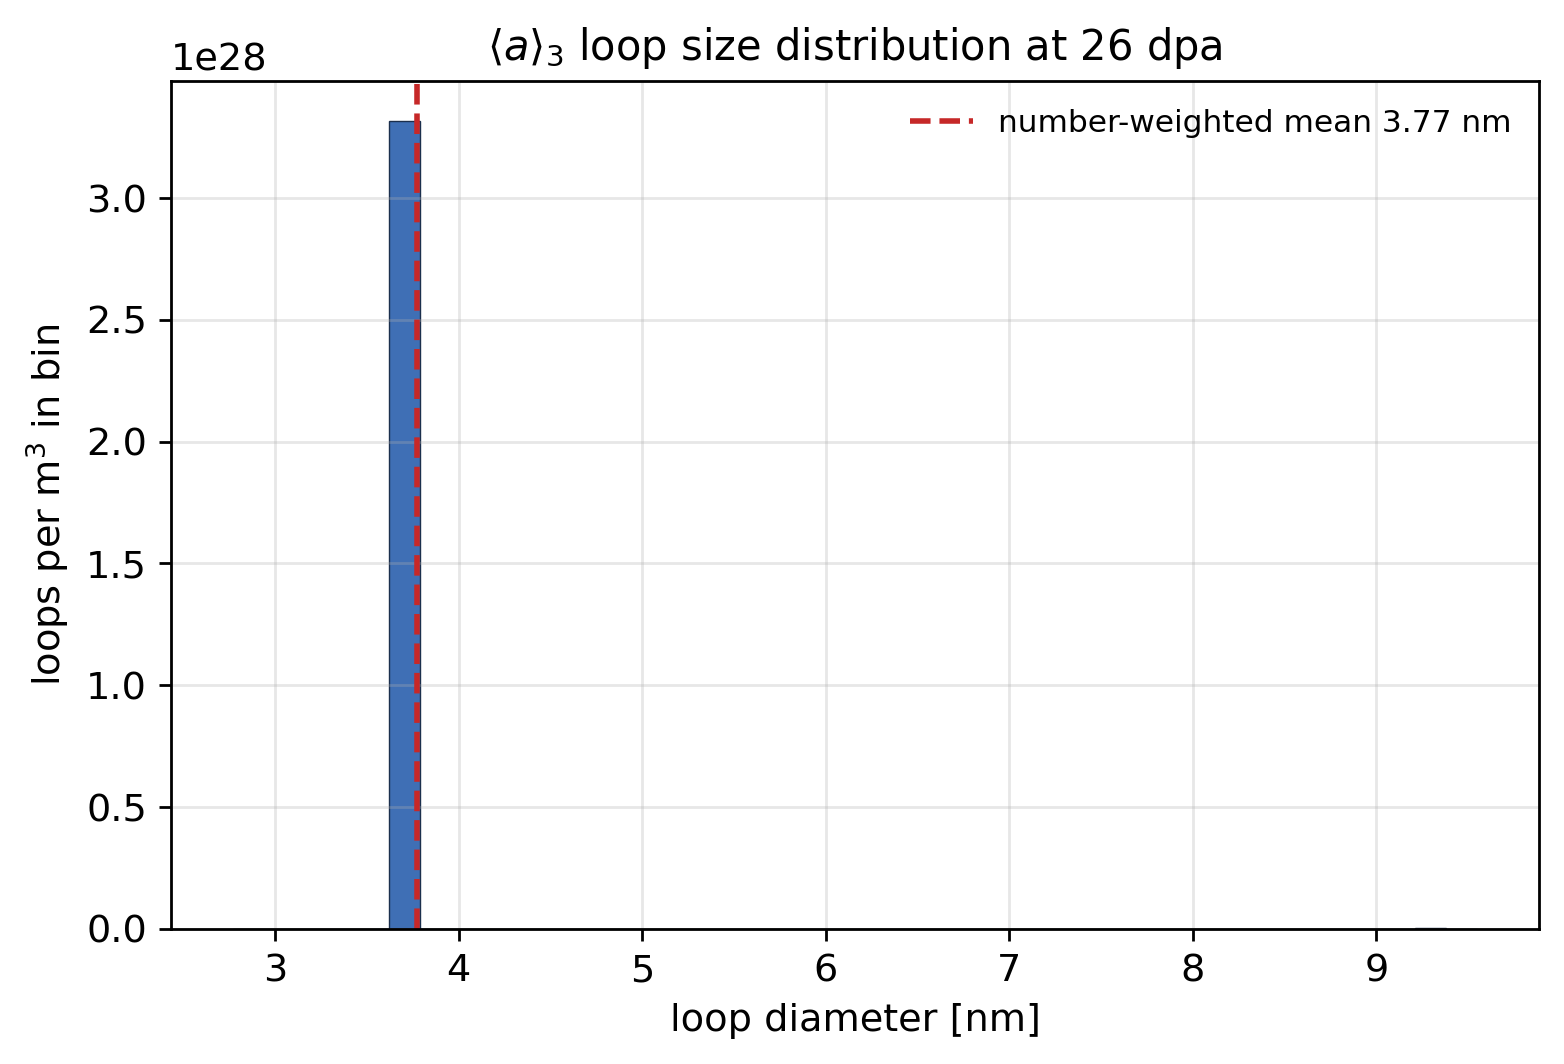
\includegraphics[width=0.45\linewidth]{figures/size_dist_a3_26dpa.png}
\end{frame}

\begin{frame}{c-Loop Size Distributions}
\centering
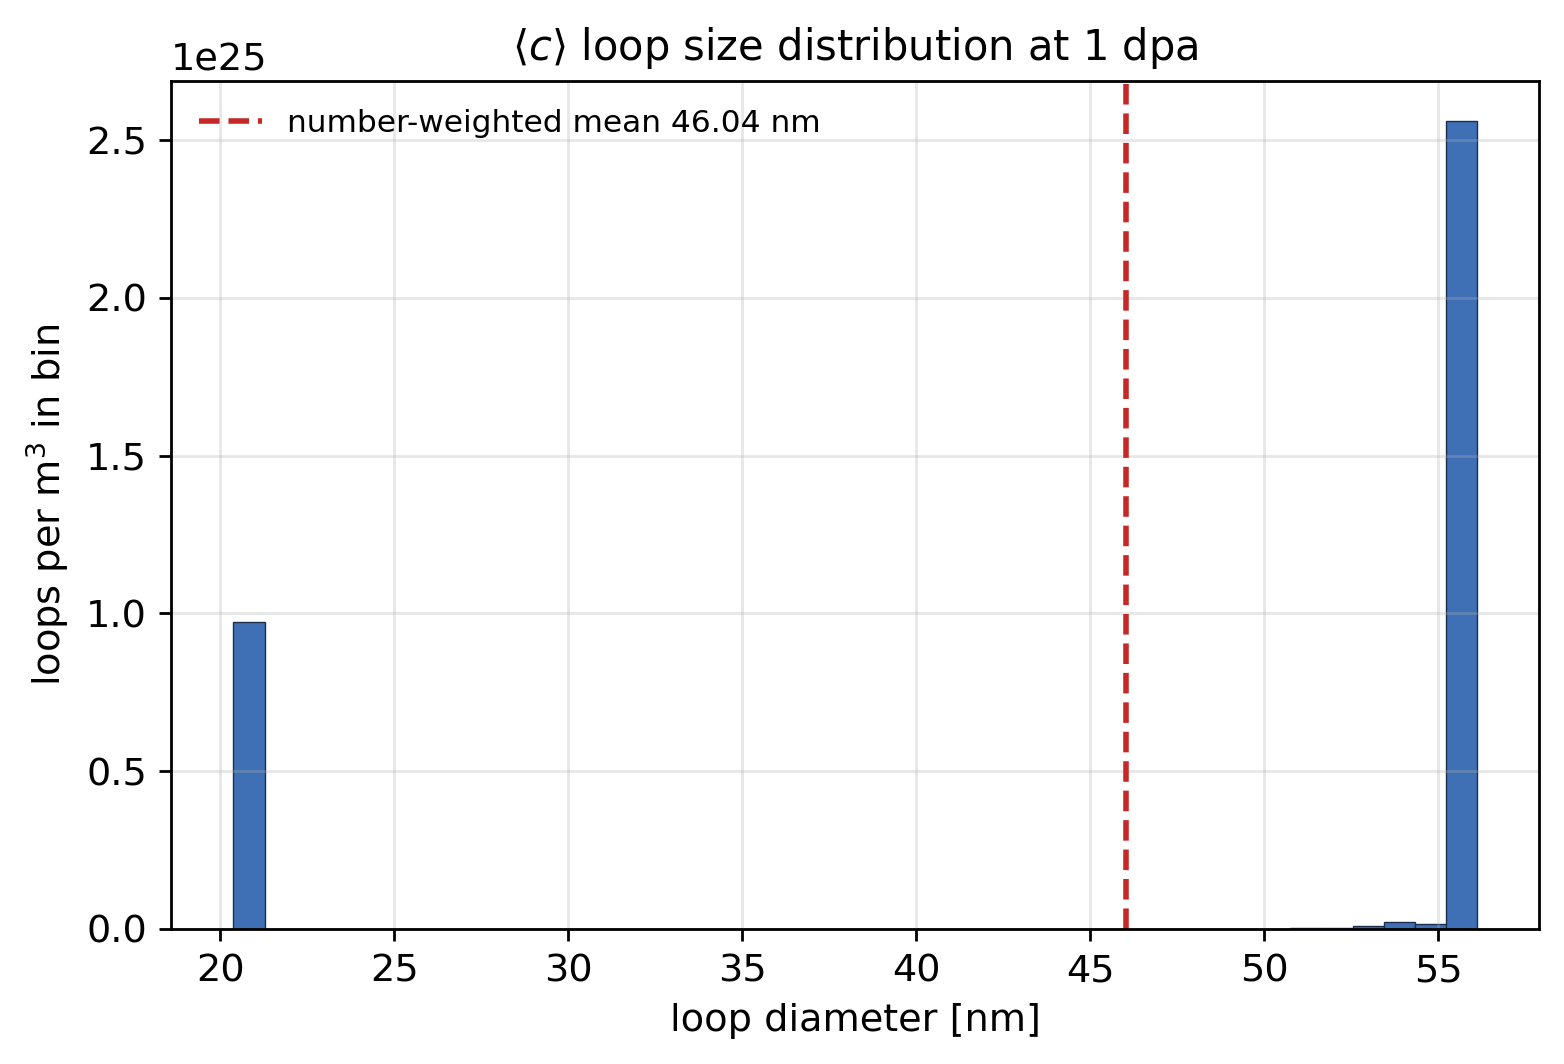
\includegraphics[width=0.45\linewidth]{figures/size_dist_c_01dpa.png}
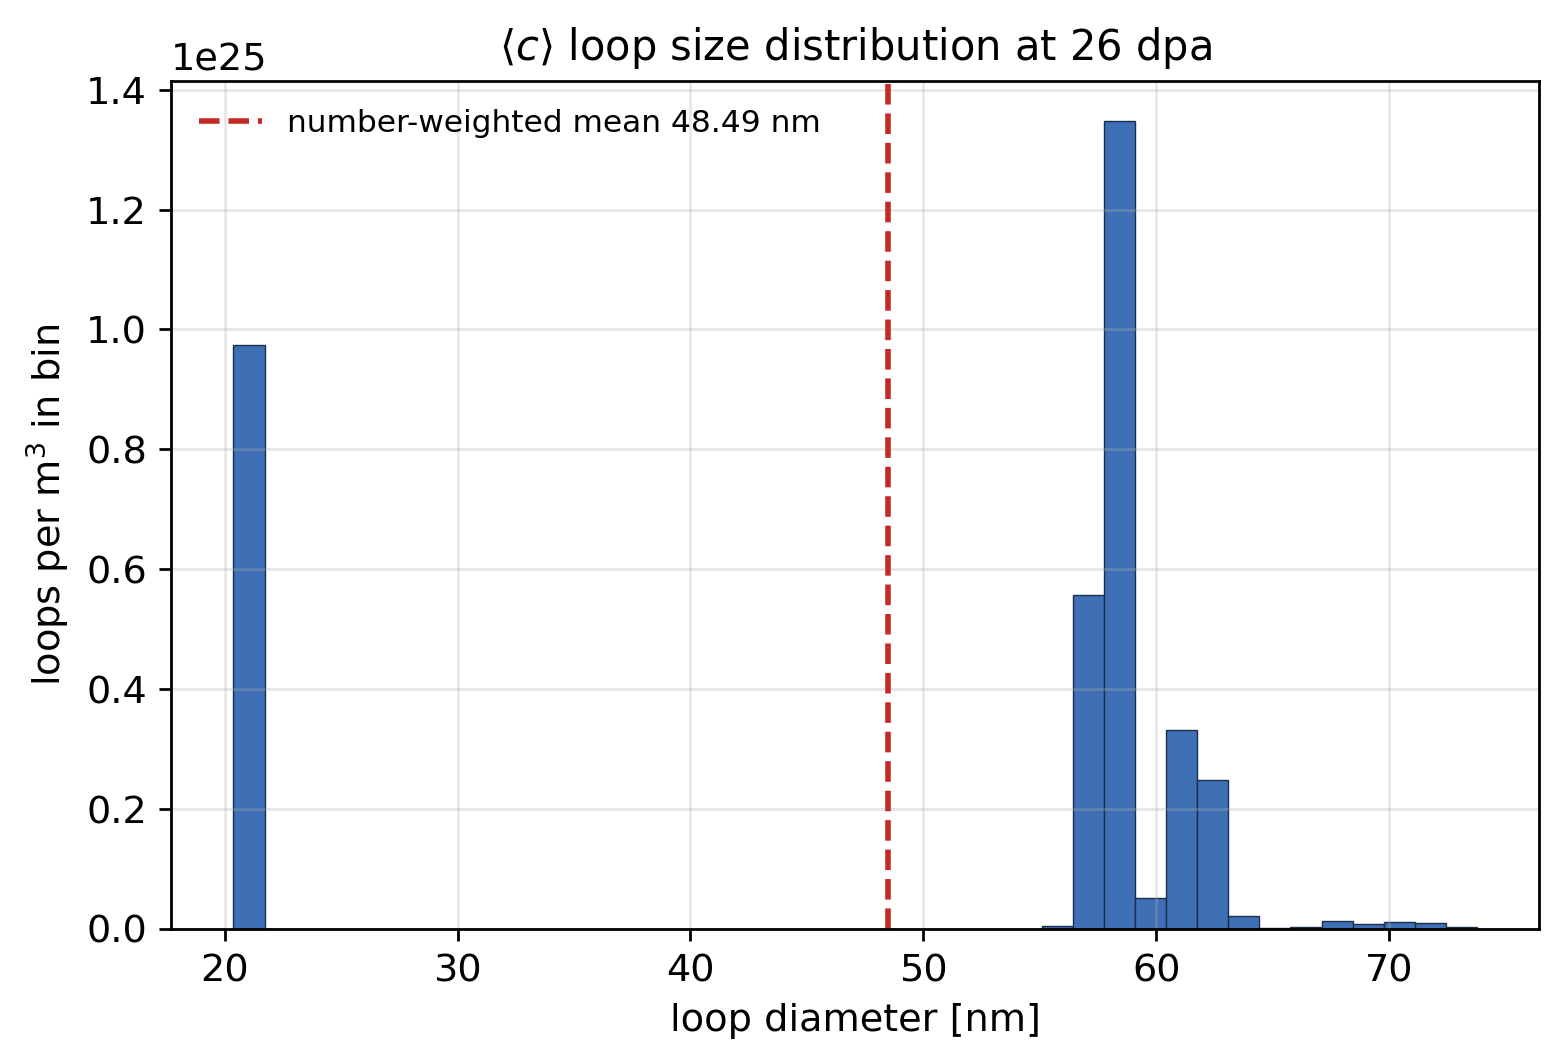
\includegraphics[width=0.45\linewidth]{figures/size_dist_c_26dpa.png}
\end{frame}

\begin{frame}{Hexagonal Single Crystal - Unstressed}
\centering
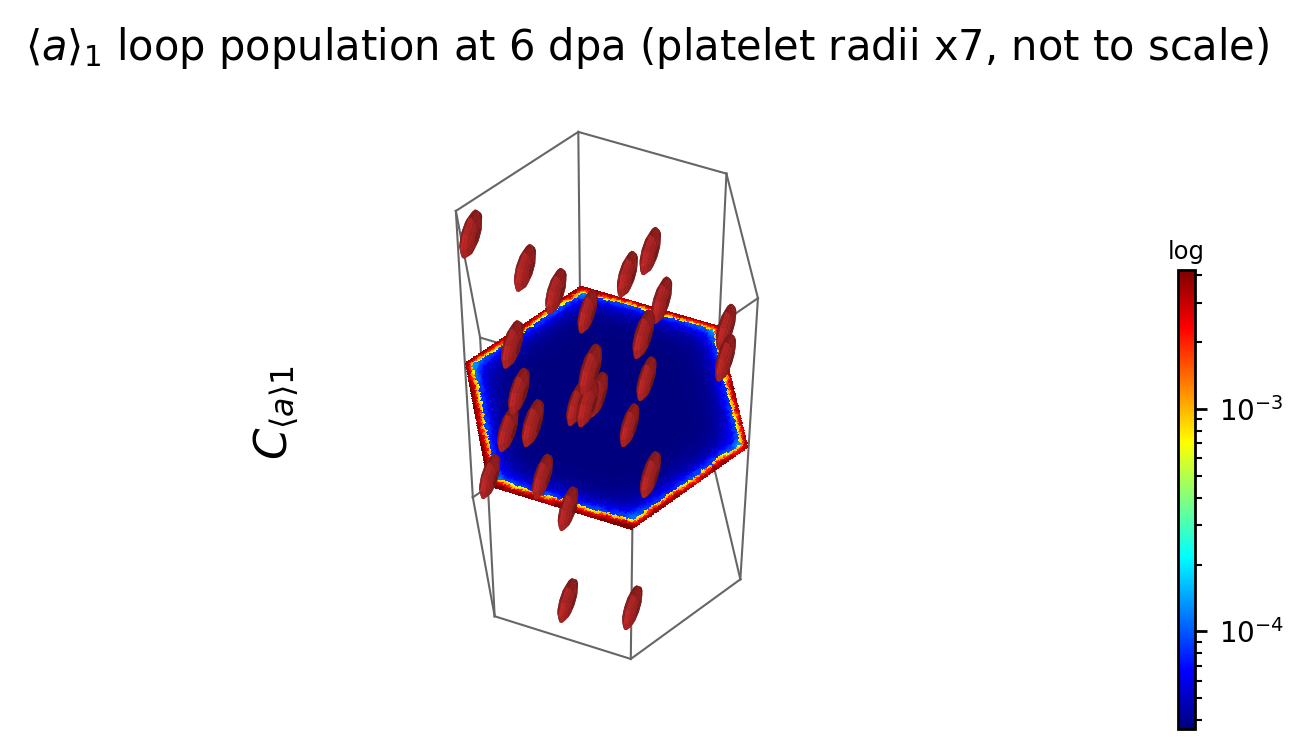
\includegraphics[width=1\linewidth]{figures/loops_a1_06dpa.png}
\end{frame}

\begin{frame}{Hexagonal Single Crystal - Unstressed}
\centering
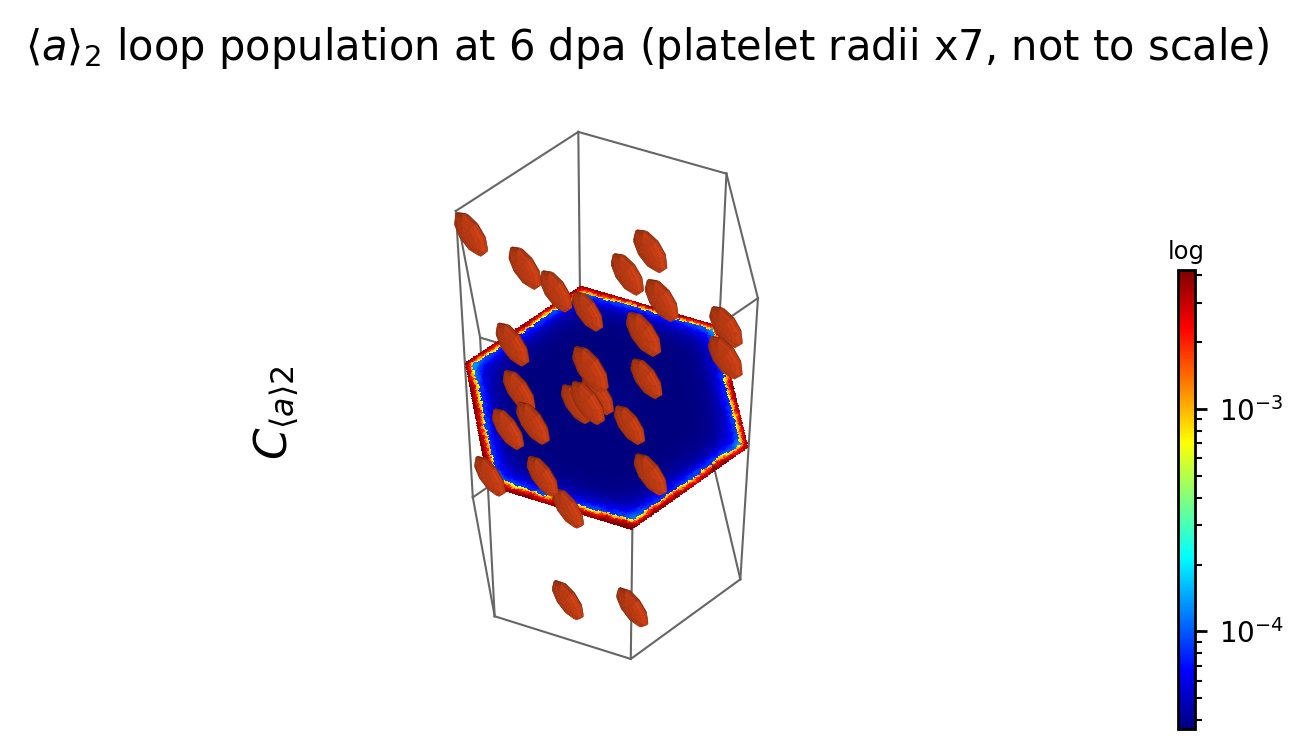
\includegraphics[width=1\linewidth]{figures/loops_a2_06dpa.png}
\end{frame}

\begin{frame}{Hexagonal Single Crystal - Unstressed}
\centering
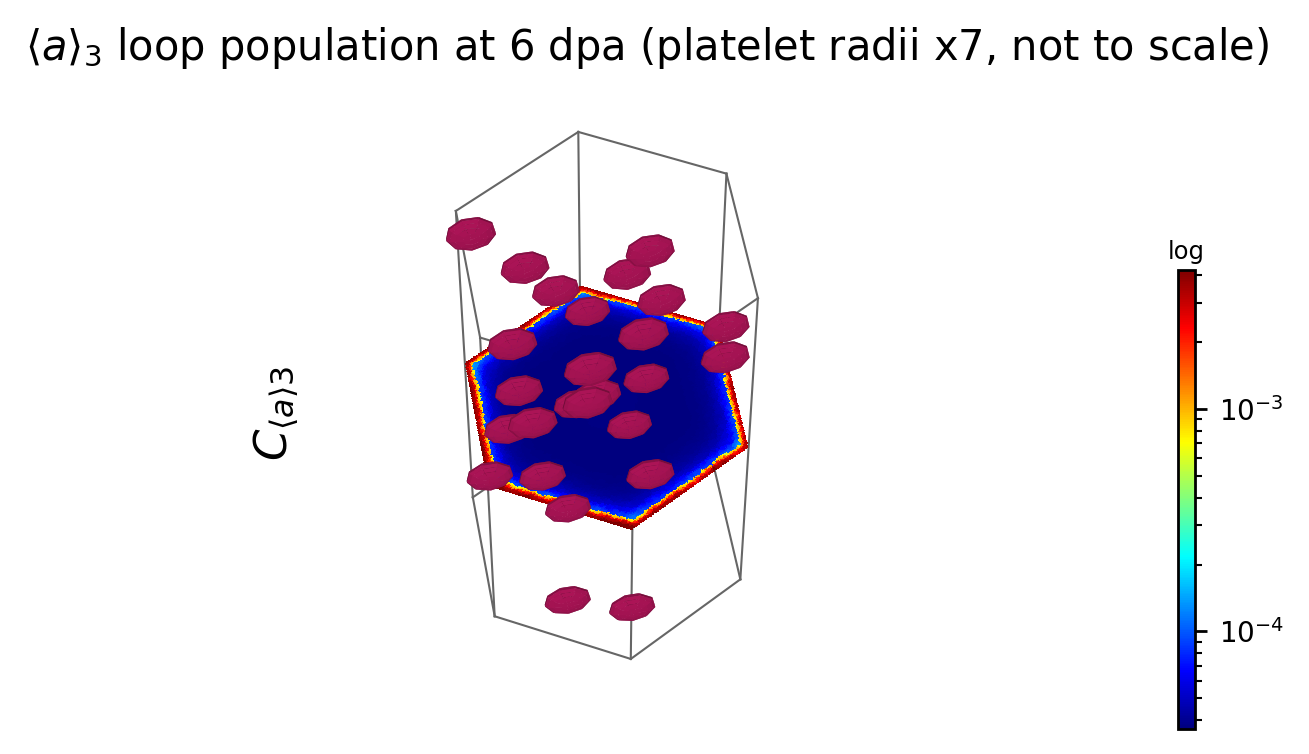
\includegraphics[width=1\linewidth]{figures/loops_a3_06dpa.png}
\end{frame}

\begin{frame}{Hexagonal Single Crystal - Unstressed}
\centering
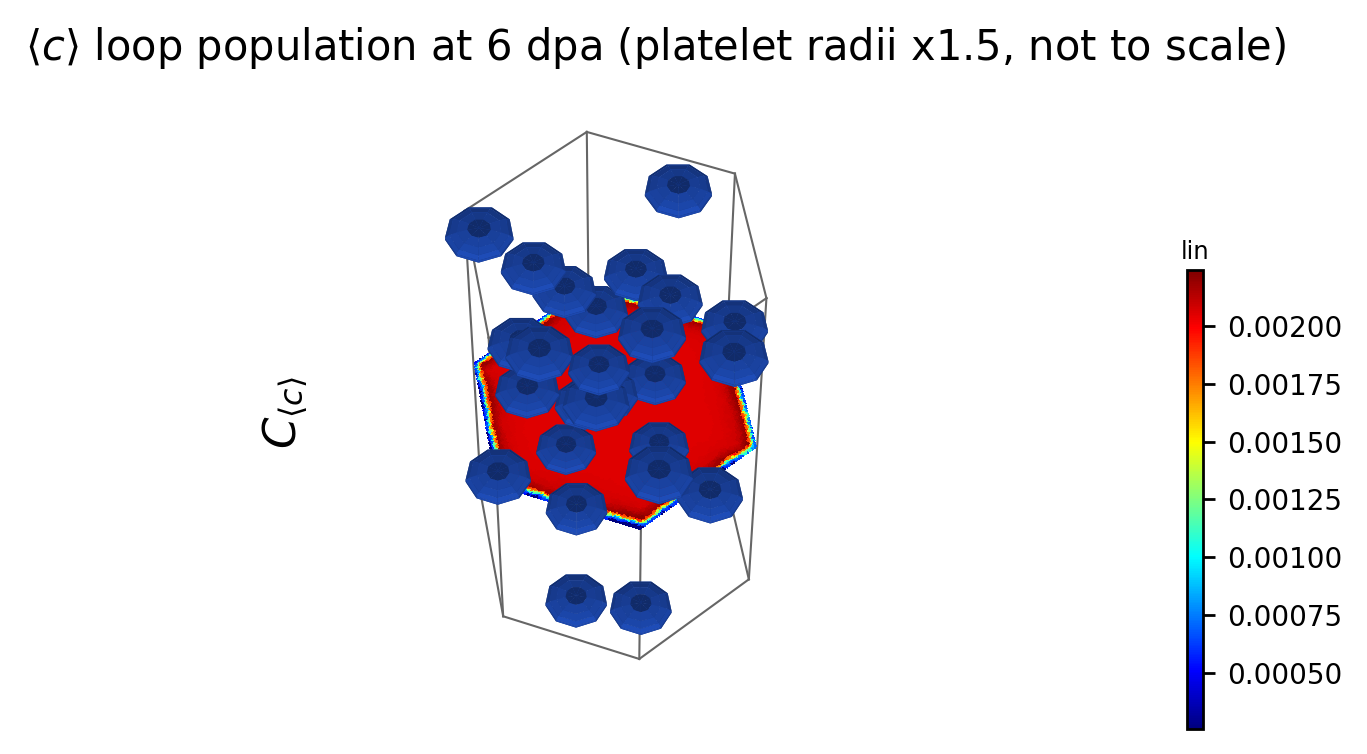
\includegraphics[width=1\linewidth]{figures/loops_c_06dpa.png}
\end{frame}


\end{document}
